%===============================================================================
% Autoři: Vladan Kudláč 2018
\chapter{Úvod}
Cílem této práce je vytvořit webovou aplikaci umožňující uživatelům upravovat videa v~internetovém prohlížeči bez nutnosti instalace dodatečných programů nebo rozšíření. Uživatel nahraje videa a obrázky ze svého zařízení nebo z~jiné služby a poté pomocí interaktivního grafického rozhraní vytvoří požadované video. Vytvořený projekt bude popsán souborem formátu XML, který zpracuje program \textit{MLT}\footnote{MLT -- sada nástrojů pro pro multimediální aplikace, \url{https://www.mltframework.org/}} na školním serveru. Dostupné možnosti úprav budou voleny tak, aby bylo možné editor použít pro tvorbu výukových videí. Editor bude vytvořen tak, aby mohl být použit jako modul pro stávající projekt \textit{prednasky.com}.
Systém bude architektury klient-server. Klient bude komunikovat se serverem pomocí zdokumentovaného API, aby mohla být implementace serveru nezávislá na klientovi a mohli v budoucnu vzniknout různé implementace klientů. Klient bude poskytovat grafické uživatelské rozhraní pomocí HTML, CSS a JavaScriptu, server bude obsluhovat požadavky, generovat XML projektů a komunikovat s~dalšími serverovými moduly. Díky této práci vznikne editor se svobodnou licencí, jako alternativa k webovým editorům s licencí ve formě předplatného a uzavřeným kódem.

Potřeby jednoduchého online video editoru vznikly při práci na portálu s výukovými videi \textit{Prednasky.com}. Při hledání řešení, které by šlo začlenit do projektu jsme zjistili, že nic takového na trhu není. Buď bylo řešení placené, nebo bylo zdarma, ale s omezenou funkčností. Ani jedno stávající řešení není s otevřeným zdrojovým kódem, které by licence dovolila použít jako komponentu projektu.

V první kapitole zmiňuji a srovnávám významné video editory, zejména v oblasti dostupných funkcí a licence. Dále zmiňuji technologie a principy uživatelského rozhraní, u kterých jsem se inspiroval stávajícími editory. Druhá kapitola je věnována návrhu řešení. Objasňuje cíl práce, způsob, jakým jsem se editor rozhodl řešit a vysvětluje zvolené technologie. Ve třetí kapitole rozebírám teoretické základy pro práci s multimédii, na kterých má práce staví. Vysvětluji způsob práce s multimediálním frameworkem MLT a možnosti práce s multimédii přímo ve webovém prohlížeči. Ve čtvrté kapitole popisuji, jakým způsobem zvolené technologie používám, jak je projekt členěn a jak je implementován. V této kapitole uvádím požadavky pro nasazení, způsob nasazení a princip fungování programu. Pátá kapitola je věnována testování uživatelského rozhraní, získávání zpětné vazby a testování kódu. V závěrečné kapitole shrnuji aktuální stav projektu, uvádím budoucí směr vývoje a další možné aplikace, které mohou na základě otevřeného API vzniknout.

\chapter{Existující řešení}
Při návrhu editoru jsem zkoumal existující videoeditory. Vybíral jsem editory známé od YouTuberů, všeobecně známé i na základě doporučení od mého vedoucího práce a známých. Stávající řešení se dají rozdělit do dvou skupin. Desktopové video editory a online video editory. Při průzkumu existujících řešení jsem se zaměřoval zejména na projekty, které mají svobodnou licenci, nebo je lze využívat bezplatně.

\section{Desktopové editory}
Mezi desktopovými video editory existuje řada bezplatných řešení s~licencemi vhodnými pro další i komerční využití. Rozhraní aplikací bývá podobné, rozsáhlé, pro jednoduché editace využívá uživatel zlomek funkcí. Nevýhodou bývá pomalá křivka učení a nutnost provozovat aplikaci na dostatečně výkoném zařízení.

Z~řešení s~otevřeným zdrojovým kódem lze vyjmenovat například projekty \textit{Shotcut}\footnote{Shotcut -- bezplatný nelineární multiplatformní editor s~otevřeným zdrojovým kódem,\\\url{https://www.shotcut.org/}} a \textit{Kdenlive}\footnote{Kdenlive -- bezplatný nelineární editor pro prostředí KDE4, \url{https://kdenlive.org/}}, které používají jako jádro framework MLT. Oba projekty používají pro zpracování multimediálních souborů framework MLT. I~v~bezplatných aplikacích lze vytvořit libovolný projekt, oproti komerčním řešení není uživatel nijak omezován. U bezplatných řešení jsem zaznamenal problémy se stabilitou, základem je průběžné ukládání projektu. Rozhraní je u obou projektů téměř stejné, obrázek \ref{img:shotcut}. Na horní liště nabídek jsou umístěny globální akce projektu, jako otevření projektu, uložení, vpřed, zpět a vyvedení projektu. Pod nabídkou je obrazovka rozdělena do několika sloupců. Levý sloupec slouží ke správě zdrojů projektu, správě filtrů u vybrané položky na časové ose a pro nastavování vlastností a parametrů. Pro přepínání zobrazení používají oba programy karty/záložky. Pravý sloupec zobrazuje náhled zdrojových souborů nebo výsledného videa. Aktuální pozici vizualizuje svislá čára na časové ose. Přehrávání náhledu se ovládá prvky přímo pod videem. Vespod je umístěna časová osa. Operace nad časovou osou jsou umístěny v liště nabídek přímo nad osou. Osa obsahuje libovolné množství stop. Zvukové stopy mají zelenou barvu, video stopy barvu modrou.
\begin{figure}[h]
	\centering
	\scalebox{0.6}{
		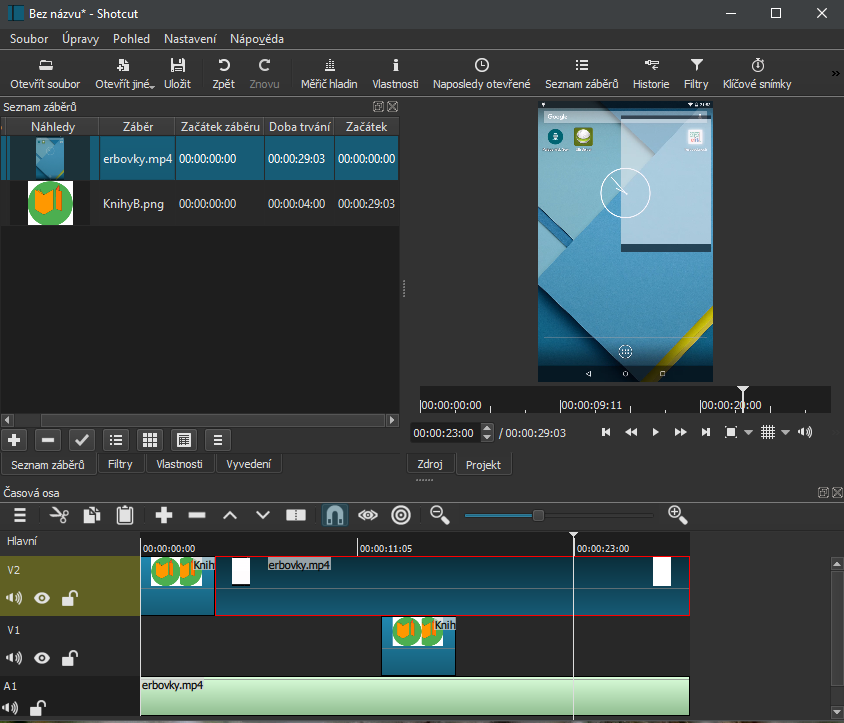
\includegraphics{obrazky-figures/shotcup.png}
	}
	\caption{Uživatelské rozhraní nelineárního video editoru Shotcut.}\label{img:shotcut}
\end{figure}

Bezplatnou aplikací nevyužívající framework MLT je například program \textit{Openshot}\footnote{Openshot -- bezplatný nelineární editor s~prostředím GTK+, \url{https://www.openshot.org/}}, který přešel na vlastní jádro. Jeho rozhraní je oproti předchozím dvou editorům velmi zjednodušené. Rozvržení zůstává stejné, pouze omezuje počet informací, které uživateli poskytuje. Nahoře se opět nacházejí akce k projektu, vlevo knihovna souborů, filtrů a přechodů, vpravo náhled s jednoznačnými ikonami a ve spodní části se nacházejí časové osy a rovněž se zde nastavují vlastnosti filtrů/přechodů. I přes zjednodušení rozhraní zde žádné funkce nechybí.

Mezi kvalitní proprietární programy se řadí program \textit{iMovie} od firmy Apple, \textit{Adobe Premiere Pro} od firmy Adobe Systems a \textit{VEGAS Movie Studio} od firmy Sony. Profesionální programy se od bezplatných liší zejména vyšší stabilitou, propracovanějšími filtry a šablonami. Licence se pohybují v~řádech tisícikorun a například Adobe nabízí svůj produkt pouze ve formě předplatného. Z těchto programů jsem vyzkoušel \textit{iMovie}. Program od firmy Apple dělí pracovní prostor do stejných skupin. Na rozdíl od předešlých programů zobrazuje v levé polovině nejen soubory k aktuálnímu projektu, ale i soubory v knihovnách. V navrhovaném řešení je rovněž potřeba řešit sdílenou knihovnu s obecnými zdroji sdílenými například s uživateli fakulty. Odlišná je aplikace filtrů. Filtry se nacházejí nad náhledem videa, jako ikony pro skupiny filtrů. Po rozkliknutí ikony se zobrazí nabídka filtrů. Uživatel nikdy nenastavuje číselné hodnoty. Nastavení filtrů je řešeno vizuálními posuvníky, kapátky a dalšími nástroji. Zajímavě řešená je časová osa, která nemá pravítko s časem. Měřítko času je na ose proměnlivé, obrázek \ref{img:imovie}. Mezi klipy je mezera, ačkoliv konec předchozího a začátek následujícího klipu je ve stejný čas. Z mého pohledu se jedná o rušivý prvek, při přehrávání ukazatel aktuálního času přeskakuje a mění svou rychlost. Na druhou stranu lze do mezer pohodlně vkládat přechody. Za zvláštní vlastnost považuji nemožnost posouvat položky po časové ose, je možné pouze měnit pořadí položek. Pokud potřebujeme mít ve videu prázdné místo, musíme zde vložit jednolitou barvu z knihovny (záložky Pozadí). Nad časovou osou chybí lišta nástrojů. Nástroje k položkám časové osy jsou dostupné skrze kontextovou nabídku vyvolanou stiskem pravého tlačítka myši nebo skrze klávesové zkratky. Video stopy jsou laděny do modrých barev, zvukové stopy do barev zelených. Z programu iMovie jsem čerpal tmavé barevné schéma.
\begin{figure}[h]
	\centering
	\scalebox{0.3}{
		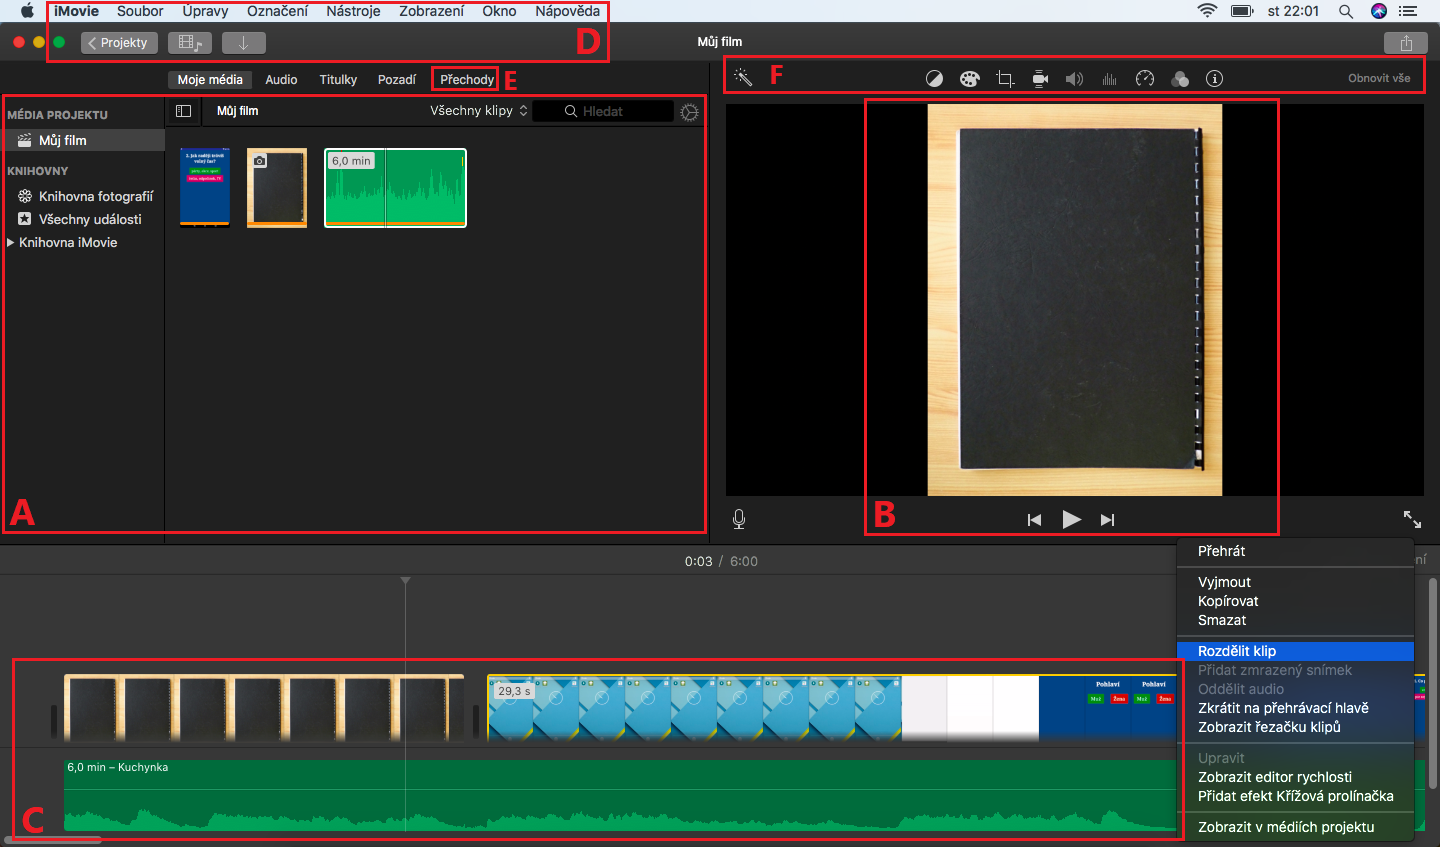
\includegraphics{obrazky-figures/iMovie.png}
	}
	\caption{Uživatelské rozhraní iMovie. Časová osa nemá jednotné měřítko.}\label{img:imovie}
\end{figure}

Zajímavým projektem mezi desktopovými aplikacemi je open source editor \textit{fwf}\footnote{fwf -- JavaScriptový FFmpeg editor, \url{https://github.com/daem-on/fwf}.} -- lineární video editor využívající knihovnu \textit{FFmpeg}\footnote{FFmpeg -- multiplatformní řešení pro nahrávání, konverzi a streamování audia a videa, \url{https://ffmpeg.org/}.}. Program je napsaný v~JavaScriptovém frameworku \textit{Vue.js}\footnote{Vue.js -- open source JavaScriptový framwork pro tvorbu uživatelských rozhraní, \url{https://vuejs.org/}.} a zkompilovaný pomocí nástroje \textit{Electron}.\footnote{Electron -- nástroj pro tvorbu desktopových aplikací za pomocí JavaScriptu, HTML a CSS, \url{https://electronjs.org/}.} Video editor má pouze základní funkce, není příliš spolehlivý, ale lze se u~něj inspirovat s~použitými technologiemi pro implementaci uživatelského rozhraní, obrázek \ref{img:fwf}.
\begin{figure}[h]
	\centering
	\scalebox{0.4}{
		\includegraphics{obrazky-figures/fwf.png}
	}
	\caption{Uživatelské rozhraní editoru \textit{fwf}, sestavené nástrojem Electron.}\label{img:fwf}
\end{figure}
Na časovou osu byla použita knihovna \textit{vis.js}.\footnote{vis.js -- JavaScriptová knihovna na vizualizaci dat, \url{http://visjs.org/}.}. \textit{Timeline} je jen jedním z vizualizačních nástrojů knihovny. Knihovna slouží k zobrazení událostí od Unixové epochy (00:00:00,000 1. ledna 1970), zatímco projekt začíná časem 0. Dále jsem z projektu použil font Source Sans Pro zveřejněnou pod svobodnou Open Font Licencí a pro ikony odnož použitého fontu Material Icons od Google (licence Apache-2.0).

\section{Webové editory}
Na webový editor jsem nezískal žádný tip. Lidé v mém okolí raději sáhli po open source editoru či stáhli placený program obsahující crack pomocí torrentu. U~webových editorů je velký rozdíl mezi placenými řešeními a neplacenými. Placených aplikací je nepřeberné množství s~mnoha funkcemi, bezplatná řešení mají zásadní omezení. Řešení s~otevřeným zdrojovým kódem a svobodnou licencí jsem nenašel žádné.

Placená řešení se funkcemi i rozhraním blíží nativním aplikacím. Z~placených editorů zmiňuji \textit{WeVideo}\footnote{WeVideo --  proprietární online editor, \url{https://www.wevideo.com}.}, \textit{Magisto}\footnote{Magisto -- proprietární online editor, \url{https://www.magisto.com/}.}, \textit{Loopster}\footnote{Loopster -- proprietární online editor, \url{https://www.loopster.com}.}, \textit{Animatron}\footnote{Animatron -- proprietární online editor s~nejdražším předplatným, \url{https://www.animatron.com}.} a \textit{Clipchamp}\footnote{Clichamp -- proprietární online editor, který lze používat s~omezeními bezplatně, \url{https://clipchamp.com}.}.

\textit{WeVideo} je poskytováno v mnoha plánech. Nejdražší varianta neomezuje velikostí souboru ani maximální délkou. Uživatelské rozhraní umožňuje pracovat s video soubory již během nahrávání na server. Náhled je generován v prohlížeči, výsledné video na serveru. Po dokončení zpracování je uživateli zaslán email. Videa vytvořená v bezplatném plánu obsahují vodoznak.

\textit{Magisto} nabízí pouze placelé plány. Nejlevnější plán limituje maximální délkou výsledného videa 2,5 minuty. Nejdražší plám má rovněž velmi limitující omezení -- 10 minut.

\textit{Loopster} nabízí ve všech plánech výstupní rozlišení 1080p. Zásadním problémem pro zpracovávání přednášek je maximální délka -- 30 minut u nejdražšího plánu.

\textit{Animatron} slouží spíše k tvorbě krátkých upoutávek a reklam. Umožňuje v nejdražším předplatném vytvořit projekt o maximální délce 10 minut. Bezplatný plán neumožňuje stažení videa, pouze vystavení videa na sociálních sítích. Při práci s editorem jsem zaznamenal problém s různou orientací stejného videa napříč editorem.

Pro nenáročné uživatele by mohl být dostačující nástroj \textit{Clipchamp Create}, který nabízí i bezplatný plán s~omezením rozlišení videí na 480p. Velikost projektu omezena není a video není opatřeno reklamním vodoznakem. Rozhraní je shodné s desktopovými programy, obrázek \ref{img:clipchamp}. Editor běží pouze v prohlížeči Google Chrome a zpracování videa probíhá na straně webového prohlížeče. Uživatel nesmí videoeditor během zpracovávání opustit. Doba zpracování videa o délce do 2 minut trvá i při rozlišení 480p cca 20 minut.
\begin{figure}[h]
	\centering
	\scalebox{0.5}{
		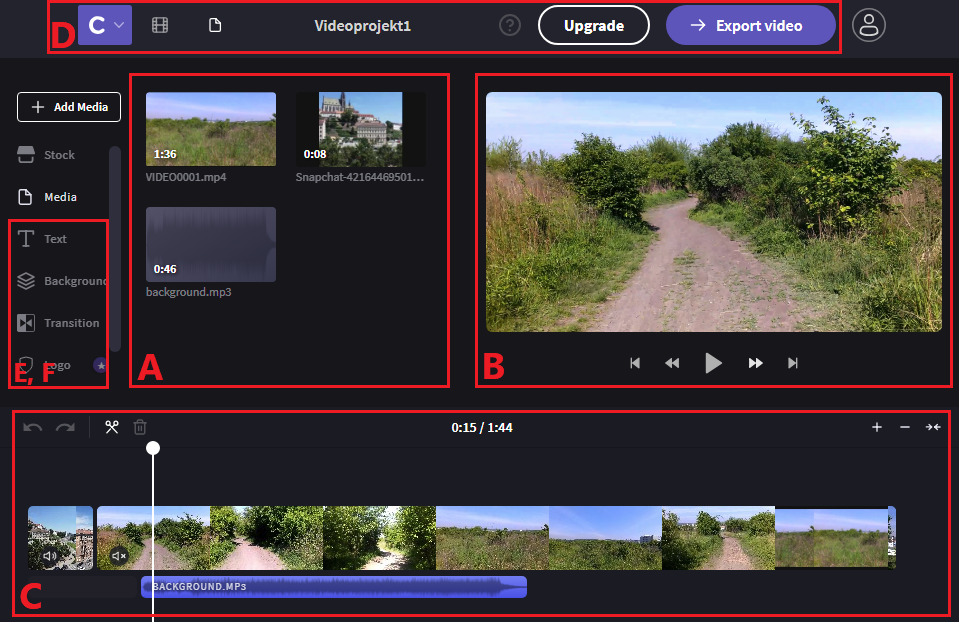
\includegraphics{obrazky-figures/clipchamp.png}
	}
	\caption{Uživatelské rozhraní nelineárního online video editoru \textit{Clipchamp Create}.}\label{img:clipchamp}
\end{figure}

Další dva editory uvádím pro úplnost, ani jeden není použitelný -- \textit{Kizoa}\footnote{Kioza -- bezplatný lineární online video editor, \url{https://www.kizoa.com}.} a \textit{Movie Maker Online}\footnote{Movie Maker Online -- bezplatný online editor, \url{https://moviemakeronline.com/}.}.

Editor \textit{Kizoa} je vytvořen v~programu \textit{Adobe Flash}, obsahuje dostatečné množství efektů, přechodů a nastavení. Vespod zobrazuje jednu časovou osu, jedná se o~lineární editor. Hlavní nevýhodou je vázanost na \textit{Adobe Flash Player}, který je dnes na ústupu a jeho podpora skončí v~roce 2020\,\cite{FlashPlayer}. Bezplatné předplatné nabídne 2 minuty videa s rozlišením 720p, nejdražší předplatné 4K video bez omezení délky.
\begin{figure}[h]
	\centering
	\scalebox{0.53}{
		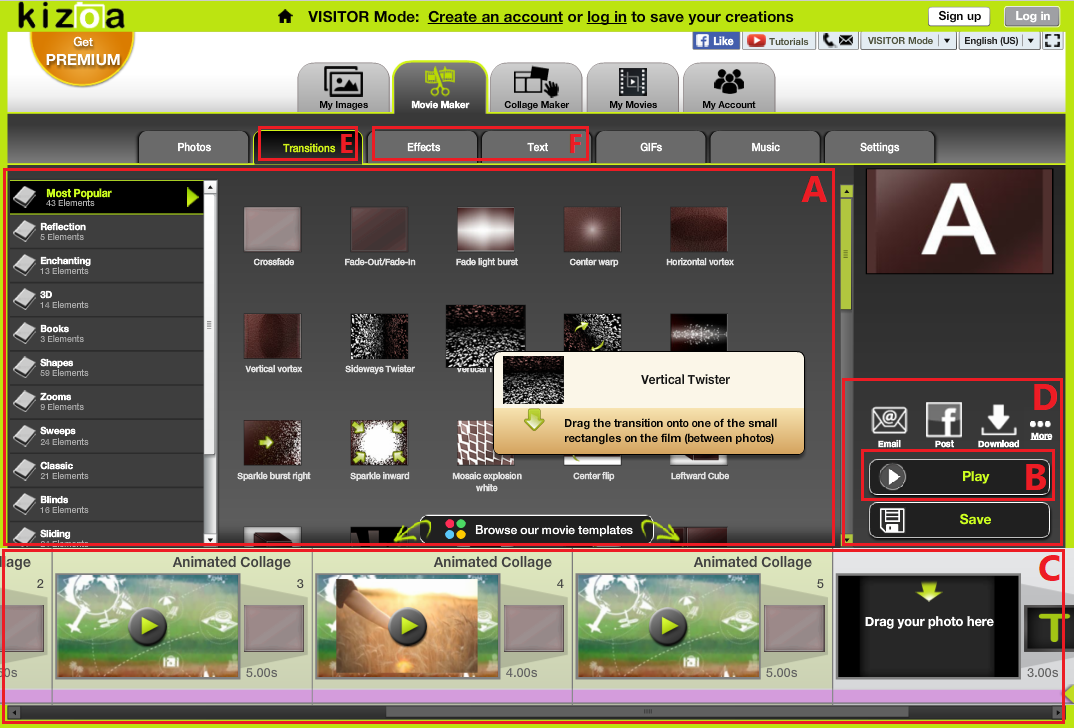
\includegraphics{obrazky-figures/kizoa.png}
	}
	\caption{Uživatelské rozhraní online lineárního video editoru Kizoa.}\label{img:kizoa}
\end{figure}

\textit{Movie Maker Online} představuje video editor s~netradičním uživatelským rozhraním. Nevyužívá zásuvných modulů a osu s~videem zobrazuje vertikálně. Jedná se o~nelineární editor, který má 4 stopy -- zvukovou, stopu s~pozadím, hlavní stopu a stopu s~překryvným textem. Přidat nebo odebrat stopu není možné. Editor je řešen jako jedna stránka, na které se pod sebou nacházejí jednotlivé kroky. Nahrávání souborů probíhá v~prvním kroku, poté se musí uživatel přesunout ke kroku 2 a provést editace. Pro uživatele desktopových aplikací se jedná o~zcela jiné rozhraní, ve kterém se budou těžko orientovat. Na rozdíl od předchozího řešení neumožňuje \textit{Movie Maker Online} projekt uložit nebo exportovat a později opětovně použít. Program lze používat bez registrace, výsledné video o rozlišení 720p je opatřeno vodoznakem a nesmí přesáhnout 10 minut. Program by měl nabízet předplatné, aktuálně ale nelze získat.
\begin{figure}[h]
	\centering
	\scalebox{0.53}{
		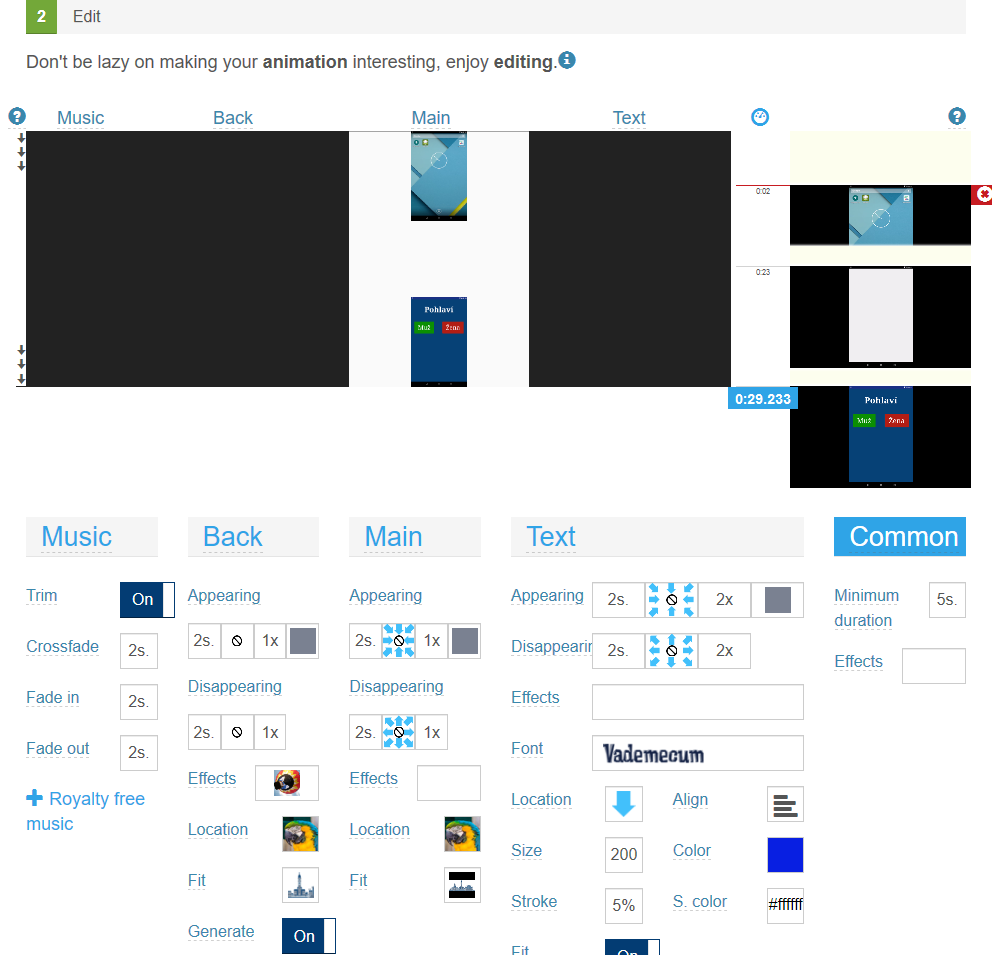
\includegraphics{obrazky-figures/moviemakeronline.png}
	}
	\caption{Uživatelské rozhraní online video editoru Movie Maker Online.}\label{img:moviemakeronline}
\end{figure}

\section{Shrnutí}
U desktopových aplikací máme široký výběr. Všechny testované programy mají podobný způsob ovládání i podobné funkce. Nemusíme se bát sáhnout po bezplatném open source řešení, i tyto programy obsahují dostatek funkcí pro kvalitní tvorbu. Neobsahují omezení na maximální rozlišení nebo délku výsledného videa. Dražší programy nabídnou propracovanější filtry a vyšší stabilitu. Při návrhu online videoeditoru je dobré zachovat rozhraní, které uživatelé znají právě z těchto aplikací. Z pohledu technologií je zajímavý jednoduchý open source lineární editor \textit{fwf}, který je napsát v JavaScriptovém framoworku \textit{Vue.js}.

Webových řešení je rovněž široký výběr. Mezi jednotlivými aplikacemi je velký rozdíl ve funkcích a zejména v omezeních výsledného videa. Z testovaných řešení nabízí neomezenou délku videa pouze program \textit{WeVideo}, \textit{Clipchamp Create}, který ale zpracovává videa v prohlížeči a \textit{Kizoa}, kterého jsem vyřadil ze srovnání kvůli vázanosti na \textit{Adobe Flash}. V rozhraních jsou větší rozdíly, než u desktopových aplikací. Uživatel desktopových editorů videa nebude mít problém s orientací v jednom z online editorů, vyjma \textit{Movie Maker Online} se zcela odlišným rozhraním. Nabízených tarify a zásadní omezení online videoeditorů srovnávám v tabulce \ref{tab:prices}.

V případě, že požadujeme online editor videí, ale zároveň potřebujeme mít svá data pod kontrolou na svém serveru, připadá v úvahu pouze program \textit{Clipchamp Create}. Program provádí veškeré operace přímo v prohlížeči. Renderování delších videí s rozlišením větší než 480p vyžaduje výkoný hardware. V tomto případě je lepší sáhnout po desktopové aplikace. Pokud chceme zpracovávat videa online, ale na našem serveru, máme smůlu.

\begin{table}[h]
    \centering
    \begin{tabular}{|l|l|l|}
    \hline
    Program   & Magisto & Animatron\\
    \hline
    Plány   & 480p, 2,5 min 230 Kč & 720p, 15 s 0 Kč\\
            & 720p, 10 min 461 Kč   & 720p, 1 min 230 Kč\\
            & 1080p, 10 min 1614 Kč & 1080p, 5 min 899 Kč\\
            &                       & 1080p, 10 min 1360 Kč\\
    \hline
    Pozn.   & Měsíční i roční předplatné. & Měsíční i roční předplatné.\\
    \hline
    \hline
    Program & Loopster                                  & WeVideo\\
    \hline
    Plány   & 1080p, 20 min, 10 GB 115 Kč               & 480p, 5 min/měs., 1 GB, 0 Kč\\
            & 1080p, 30 min, 20 GB 230 Kč               & 720p, 30 min/měs., 20 GB, 230 Kč\\
            & 1080p, 30 min, 100 GB 2975 Kč / 3 měs.    & 4K, neomezeno 369 Kč\\
            &                                           & 4K, 3 uživ. 1383 Kč + 922 Kč/uživ.\\
    \hline
    Pozn.   & Roční předplatné.                         & Měsíční i roční předplatné.\\
            & Poslední plán účtován čtvrtletně.         & Poslední plán je multilicence.\\
    \hline
    \end{tabular}
    \caption{Přehled tarifů placených online video editorů. Pokud není uvedeno jinak, cena je za měsíc. Videa delší než 30 minut nabízí pouze WeVideo.}
    \label{tab:prices}
\end{table}

\chapter{Návrh řešení}
Hlavním cílem práce je vytvořit videoeditor, který bude fungovat ve všech moderních prohlížečích a výsledné zpracování videa nebude probíhat na straně klienta. K dosažení těchto cílů bude za nutné vytvořit webovou aplikaci. Stejně jako stávající řešení by i tento editor měl provádět veškeré úkony pomocí JavaScriptu a asynchronních požadavků, bez nutnosti znovu načítat celou stránku. Vzhledem ke komplexnosti uživatelského rozhraní není vhodné zvolit čistý JavaScript. Vyplatí se sáhnout po JavaScriptovém frameworku, usnadňují časté operace, udržují dobré návyky a pomáhají vytvořit čistý kód.

Nejpoužívanějšími\footnote{Wappalyzer -- doplněk prohlížeče pro analýzu webových technologií, data od uživatelů agreguje do statistik, \url{https://www.wappalyzer.com/categories/javascript-frameworks}.} frameworky jsou: React, Backbone.js, RequireJS, AngularJS, nebo třeba Vue.js (používané programem \textit{fwf}). Z těchto frameworků jsem vybral React, který je zároveň i šablonovacím systémem a má kvalitní dokumentaci. Šablonovací systém používám zejména k rozdělení uživatelského rozhraní na komponenty.

Webová aplikace bude potřebovat i serverovou část, na kterou klient nahraje soubory, popíše serveru operace nad soubory a dá pokyn pro vyhotovení výsledného videa. Tuto architekturu označujeme jako klient-server. Mezi klientem a serverem je nutné komunikovat. Pro výměnu dat po síti musejí obě části používat dohodnutý serializační formát. JavaScript nejčastěji používá \textit{XML} nebo \textit{JSON}. \textit{JSON} (JavaScriptový objektový zápis) je novější a zápis ve formátu \textit{JSON} je validním kódem JavaScriptu. \textit{XML} (rozšiřitelný značkovací jazyk) na druhou stranu umožňuje přenos binárních dat. Se serverem bude komunikovat JavaScript, volba formátu \textit{JSON} je tedy výhodná.

Sever bude mít za úkol 2 činnosti. Nejprve bude muset uživateli poskytnout soubory s HTML, CSS a JavaScriptem a poté reagovat na JavaScriptové asynchronní požadavky. Při návrhu jsem se rozhodoval mezi implementací serveru pomocí jazyka PHP a pomocí Node.js. Jazyk PHP vznikal v době statických stránek a osobních webů, Node.js je obvykle spojován se single page aplikacemi. Node.js jsem si vybral právě protože plánuji vytvořit single page aplikaci, kvůli možnosti používat stejný jazyk pro klientskou i serverovou část a také kvůli asynchronnímu přístupu k blokujícím operacím. Po PHP bych naopak sáhl při tvorbě e-shopu, blogu či informačního systému.

Server bude pro klienta dosputný skrze rozhraní (API). Rozhraní bude sloužit k vyvolání akcí na serveru i k získávání dat. Existuje více koncepcí pro komunikaci a tvorbu API, například \textit{XML-RPC}, \textit{SOAP} nebo \textit{REST}. \textit{XML-RPC} a \textit{SOAP} používají jako serializační formát pro výměnu dat \textit{XML}, kvůli JavaScriptu na střaně klienta i serveru jsem ovšem zvolil \textit{JSON}. \textit{REST} je způsob komunikace na základě HTTP požadavků. \textit{REST} není na HTTP vázaný, ale není praktický důvod používat odlišný protokol. Výchozím serializačním formátem pro výměnu dat je JSON, ovšem lze používat například i \textit{XML}.

Multimediální soubory bude potřeba zpracovávat. \textit{Clipchamp Create} provádí zpracování na straně klienta ve webovém prohlížeči. Webový prohlížeč ani webové technologie ale nejsou navrženy na renderování videí, \textit{Clipchamp} vyvádí video déle, než bych byl ochotný čekat. Editor byl navržen aby zpracovával videa na serveru. K tomu může sloužit program \textit{FFmpeg} nebo \textit{MLT}. Program \textit{FFmpeg} používá například editor \textit{fwf} nebo Android aplikace \textit{Video Editor using FFmpeg}\footnote{Video Editor using FFmpeg -- open source editor videa pro android, \url{https://github.com/bhuvnesh123/FFmpeg-Video-Editor-Android}.}. \textit{FFmpeg} se používá skrze příkazový řádek. Každá operace představuje jeden příkaz (zkrátit video, přidat efekt, spojit videa). Na přadí operací záleží. Projekt by byl popsán souborem s posloupností příkazů pro FFmpeg, případně jedním dlouhým příkazem. Multimediální framework \textit{MLT} rovněž nabízí své nástroje skrze příkazový řádek. Projekt je možné popisovat posloupností příkazů a také pomocí serializačního formátu \textit{XML}. Celý projekt se popíše entitami \textit{XML} a programu \textit{MLT} se poté pouze předá \textit{XML} sobor. \textit{XML} soubor bude uložen po celou dobu na serveru a server jej bude editovat na základě požadavků klienta. \textit{REST API} je bezstavové, požadavek musí být úplný a stav projektu je uložen v \textit{XML} souboru projektu.

\section{Návrh uživatelského rozhraní}
Cílovou skupinou jsou počítačově gramotní uživatelé, kteří někdy používali program na editování videa. Rozhraní je voleno tak, aby připomínalo klasické desktopové aplikace a pomohlo uživatelům se zorientovat. Typickou úlohou pro videoeditor bude sestříhat záznam přednášky do výukového videa nebo vytvořit tutoriál ze záznamu z kamery nebo obrazovky. Aplikace bude využívána na na počítačích a noteboocích, není nutné přizpůsobovat rozhraní obrazovkám mobilních zařízení. Ovládání bude pomocí klávesnice a myši, dotekové obrazovky se sice nepředpokládají, ale ani nevylučují.

Po načtení hlavní stránky se zobrazí úvodní stránka s možností vytvořit nový projekt. Stránka bude do budoucna připravena na rozšíření o další možnosti, jako jsou šablony, autentizace uživatelů, či seznam vlastních projektů. Pro zahájení editace uživatel zvolí \textit{Vytvořit nový projekt}, obrázek \ref{img:novy-projekt}.
\begin{figure}[h]
	\centering
	\scalebox{0.5}{
		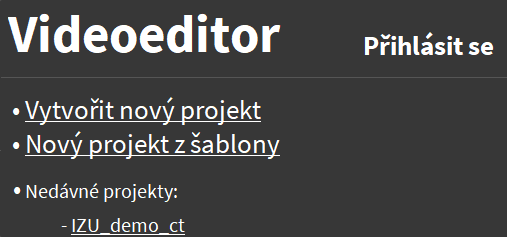
\includegraphics{obrazky-figures/novy_projekt.png}
	}
	\caption{Úvodní obrazovka pro vytváření nových projektů.}\label{img:novy-projekt}
\end{figure}

Po vytvoření nového projektu se uživatel ocitne v rozhraní pro tvorbu videí. Aplikace je řešena jako single page aplikace. Uživatel po celou dobu pracuje na jedné obrazovce a i při dialozích je editor překryt pouze částečně, tak, aby měl uživatel pocit, že má svůj projekt po celou dobu pod kontrolou. Při návrhu uživatelského rozhraní editoru jsem se nejvíce inspiroval desktopovou aplikací \textit{iMovie}, \textit{Shotcut} a online nástrojem pro úpravu fotografií -- \textit{Photopea}\footnote{Photopea.com -- bezplatný editor fotografií, \url{https://www.photopea.com/}}.

Uživatelské rozhraní editoru je rozděleno do 4 částí. Rozložení bylo navrženo a odzkoušeno na drátěném modelu, obrázek \ref{img:wireframe}.
\begin{figure}[h]
	\centering
	\scalebox{0.3}{
		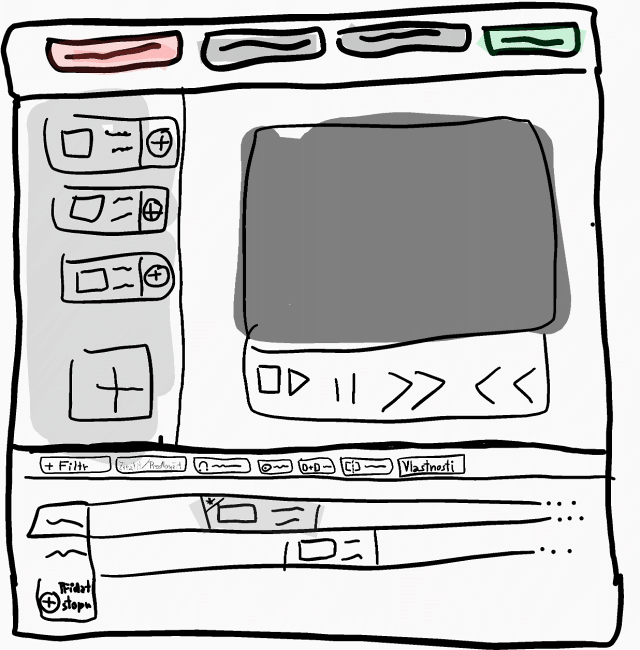
\includegraphics{obrazky-figures/wireframe}
	}
	\caption{Drátěný model uživatelského rozhraní.}\label{img:wireframe}
\end{figure}
Na základě drátěného modelu byl zhotoven prototyp hlavního uživatelského rozhraní, obrázek \ref{img:mockup}.
\begin{figure}[!h]
	\centering
	\scalebox{0.6}{
		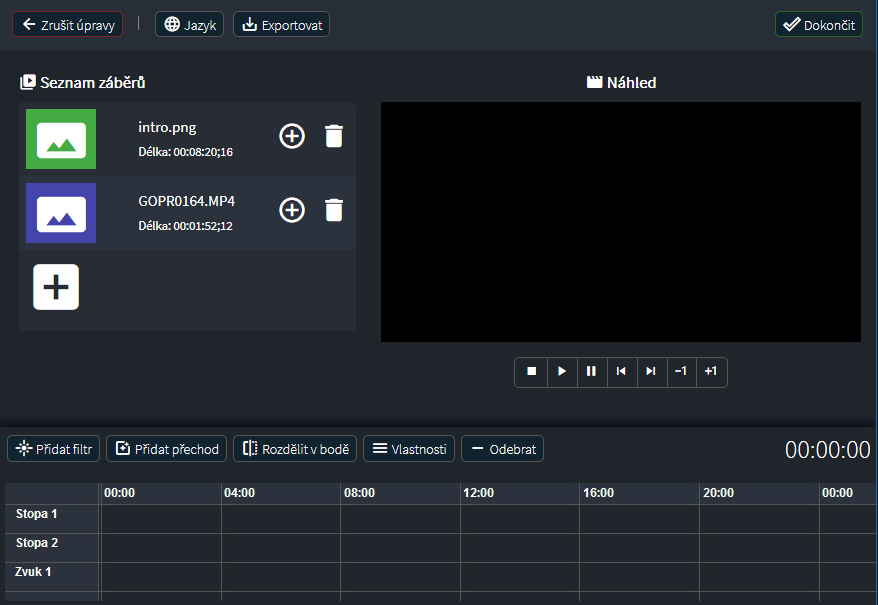
\includegraphics{obrazky-figures/mockup.png}
	}
	\caption{Prototyp uživatelského rozhraní.}\label{img:mockup}
\end{figure}

U horního obraje obrazovky se nachází panel nástrojů pro globální akce nad projektem -- zrušit úpravy nebo vyvést (dokončit) projekt. Do budoucna zde bude možnost přepínat jazykovou mutaci a možnost exportu nebo výmazu dat.

Operace nad videi jsou členěny do 3 částí, tomu odpovídá a členění uživatelského rozhraní. V~levé části je seznam zdrojového materiálu (videí, obrázků, aj.), který je možné v~projektu použít. S~položkami seznamu se zdrojovým materiálem se pracuje přímo. Dostupné operace jsou zobrazeny po celou dobu. Pod poslední položkou se nachází tlačítko na přidání materiálu, případně je možné použít přetažení souboru do této oblasti. V~seznamu zdrojů je možné nahrávat obrázkové a video soubory. Podporované formáty video souborů jsou shodné s~formáty, které podporuje multimediální framework FFmpeg. Z~obrázkových souborů je podporován formát PNG a JPEG obrázek. Obrázek \ref{img:ucd-zdroj} zobrazuje diagram případů užití pro práci se zdrojovým materiálem.
% [Uživatel]-(Nahrát video nebo obrázek),
% [Uživatel]-(Odebrat video nebo obrázek),
% [Uživatel]-(Vložit video na konec časové osy),
% [Uživatel]-(Vložit obrázek na konec časové osy),
% (Vložit obrázek na konec časové osy)>(Nastavit dobu trvání),
\begin{figure}[h]
	\centering
	\scalebox{0.4}{
		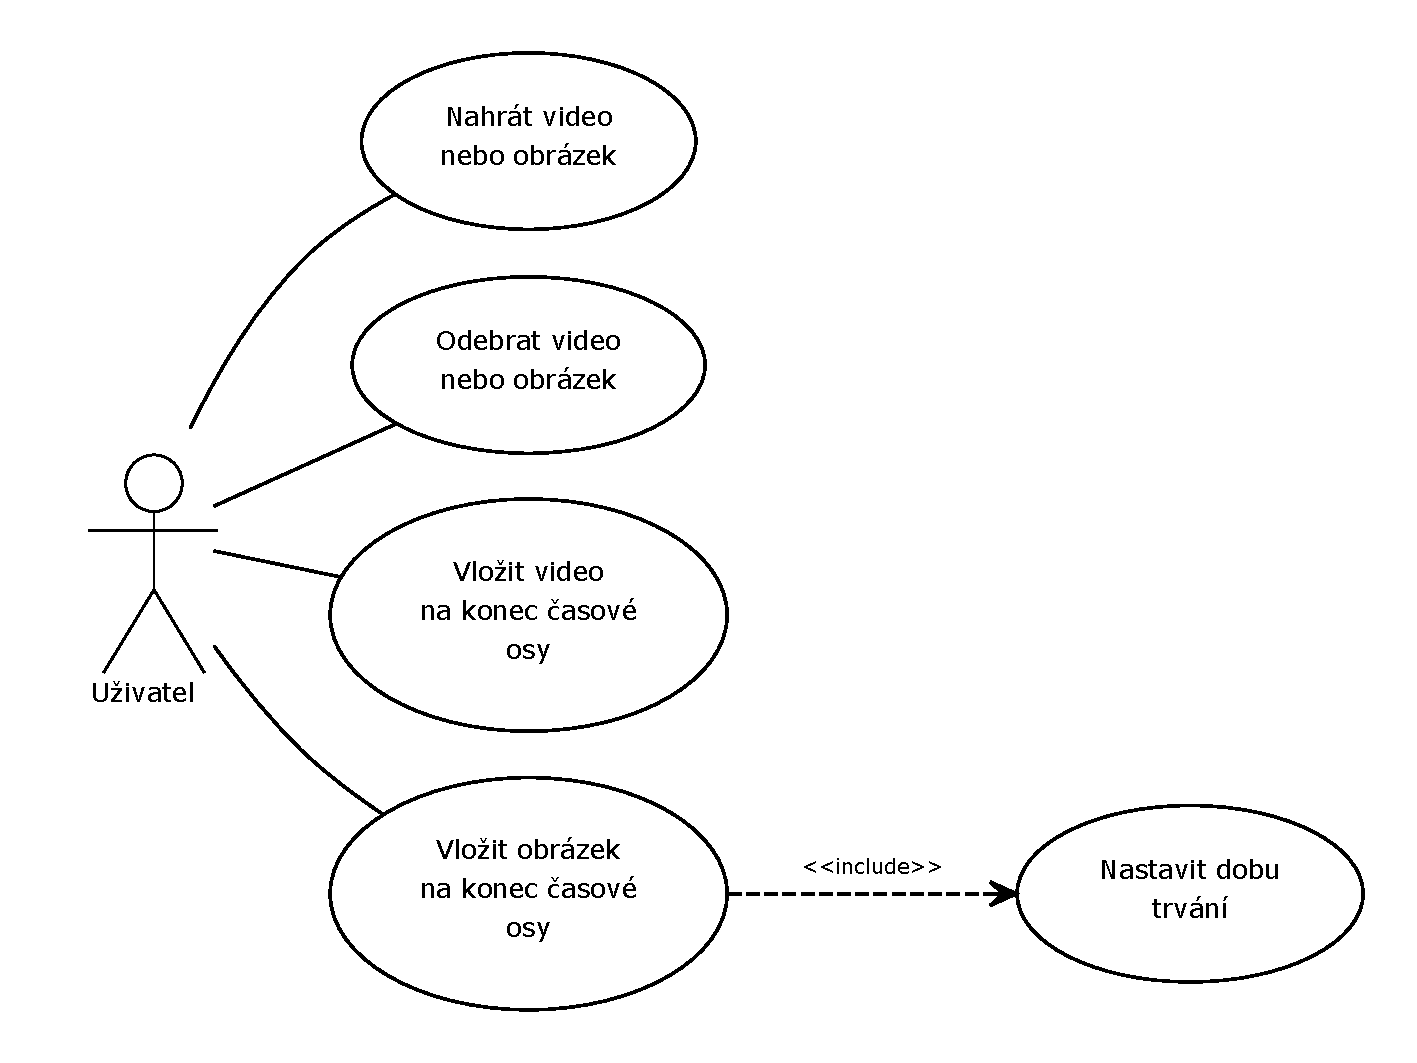
\includegraphics{obrazky-figures/ucd-zdroje.pdf}
	}
	\caption{Diagram případů užití pro práci se zdroji.}\label{img:ucd-zdroj}
\end{figure}

V~pravé polovině se nachází přehrávač předběžného náhledu výsledného videa. Přehrávač náhledu se ovládá tlačítky umístěnými přímo pod přehrávačem (přehrát, zastavit, skok na začátek nebo konec, skok na začátek nebo konec aktuální položky). Přehrávač přehrává pouze soubory umístěné na časové ose, nezobrazuje náhledy zdrojového materiálu. Aktuální pozici přehrávače udává ukazatel na časové ose. Přehrávání lze spustit původní rychlostí a pozastavit. K~manipulaci s~pozicí ve videu slouží skok na událost vpřed/vzad, který přesune ukazatel na nejbližší začátek nebo konec položky libovolné stopy, diagram případů užití zobrazuje obrázek \ref{img:ucd-prehravac}.
% [Uživatel]-(Spustit přehrávání),
% [Uživatel]-(Pozastavit přehrávání),
% [Uživatel]-(Skok na událost vpřed nebo vzad),
% [Uživatel]-(Další nebo předchozí snímek),
\begin{figure}[!h]
	\centering
	\scalebox{0.4}{
		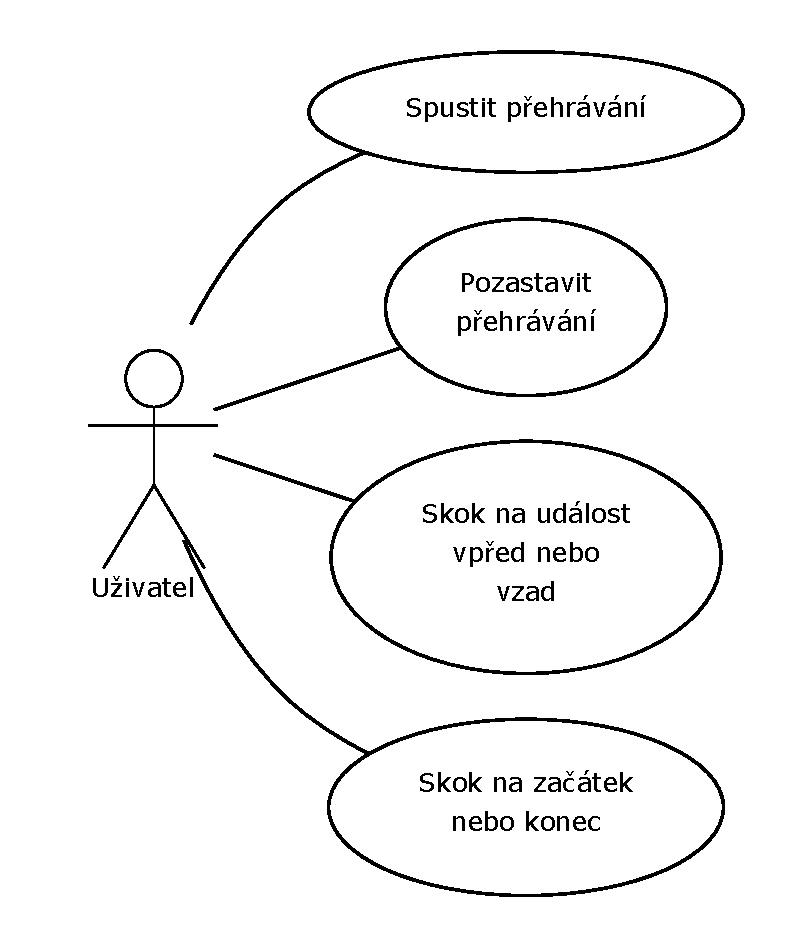
\includegraphics{obrazky-figures/ucd-prehravac.pdf}
	}
	\caption{Diagram případů užití pro práci s~přehrávačem náhledu.}\label{img:ucd-prehravac}
\end{figure}

Ve spodní části je časová osa se zvukovými a obrazovými stopami. Časová osa zobrazuje pod sebou stopy v~pořadí, v~jakém byly vytvořeny. Stopy se přidávají a odebírají podle potřeby. Pokud uživatel uchopí položku a přetáhne ji pod poslední video/audio stopu, vytvoří se nová. Původní návrh počítal se zobrazováním názvů stop a manuálním přidávání stop. Po testování jsem se rozhodl odstínit uživatele od stop a nabídnout mu pracovní plochu, kde může přesouvat položky i vedle sebe, bez nutnosti řešit stopy. Položky se na časovou osu přidávají ze seznamu materiálu tlačítkem plus u~materiálu. Posun položek na časové ose se provede uchopením prvku a přetažením na nové místo, přesun na jinou časovou se provádí přetažením na jinou osu stejného typu. Uchopením položky za okraj lze měnit začátek nebo konec. U~každé položky je náhledový obrázek a textové informace o položce. S~vybranou položkou lze pracovat tlačítky na listě nástrojů u~horního okraje časové osy. V~aplikaci jsou dvě lišty nástrojů, globální akce a akce s~časovou osou. Pokud je na položku aplikován alespoň jeden filtr, zobrazí se v jejím levém horním rohu \uv{nálepka} s ikonou filtru. Časovou osu lze přibližovat a oddalovat tlačítky v~liště nástrojů časové osy. Pokud je časová osa přiblížena natolik, že není možné zobrazit všechny prvky časové osy, lze osu posouvat do stran uchopením prázdného místa na ose a přetažením osy do stran. V~novém projektu je k~dispozici prázdná zvuková a video stopa. Ukazatel aktuálního času lze uchopit a přesunout. V~čase ukazatele se bude přehrávat náhled videa a v~tomto čase lze provést střih videa, diagram případů užití -- obrázek \ref{img:ucd-osa}.
% [Uživatel]-(Přiblížit časovou osu),
% [Uživatel]-(Posunout časovou osu do stran),
% [Uživatel]-(Přidat nebo odebrat časovou osu),
% [Uživatel]-(Nastavit pozici ukazatele)
\begin{figure}[h]
	\centering
	\scalebox{0.4}{
		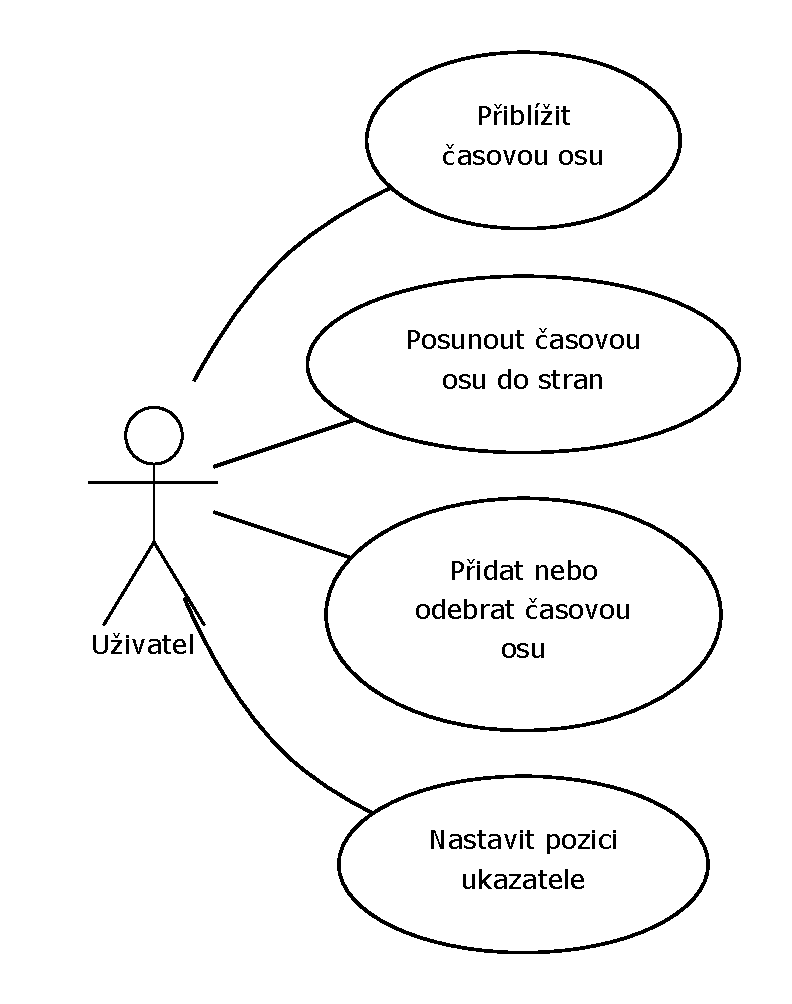
\includegraphics{obrazky-figures/ucd-osa.pdf}
	}
	\caption{Diagram případů užití pro práci s~časovou osou.}\label{img:ucd-osa}
\end{figure}

Po vybrání položky (videa nebo obrázku) na časové ose jsou k~dispozici v~panelu nástrojů časové osy následující akce. Položku lze smazat, okolní položky zůstávají, přechody se zruší. Lze přidat filtr obrazu (text, HTML překrytí, jas, kontrast, odstín, světlost, sytost, vyvážení bílé, otočit, velikost, poloha, ořezání, průhlednost, ostrost) nebo filtr zvuku (ztišit, zesílit/zeslabit). Přidat přechod prolnutí mezi 2 položkami, položky s~přechody se při přesouvání chovají jako celek. Dále lze zobrazit souhrnné vlastnosti. Následující úkony se neprovádí přes panel nástrojů --  a začátek nebo konec video souboru či délku obrázku lze změnit uchopením okraje položky a táhnutím na požadovanou pozici. Akce s vybranou položkou zobrazuje diagram případů užití na obrázku \ref{img:ucd-polozky}.
% [Uživatel]-(Posunout na časové ose),
% [Uživatel]-(Přesunout na jinou časovou osu),
% [Uživatel]-(Vybrat pro práci),
% [Uživatel]-(Změnit začátek nebo konec ořezem),
% [Uživatel]-(Rozdělit v bodě na 2 části),
% (Vybrat pro práci)<(Odstranit z časové osy),
% (Vybrat pro práci)<(Přidat filtr),
% (Vybrat pro práci)<(Přidat přechod mezi 2 položkami),
% (Vybrat pro práci)<(Zobrazit vlastnosti),
\begin{figure}[!h]
	\centering
	\scalebox{0.4}{
		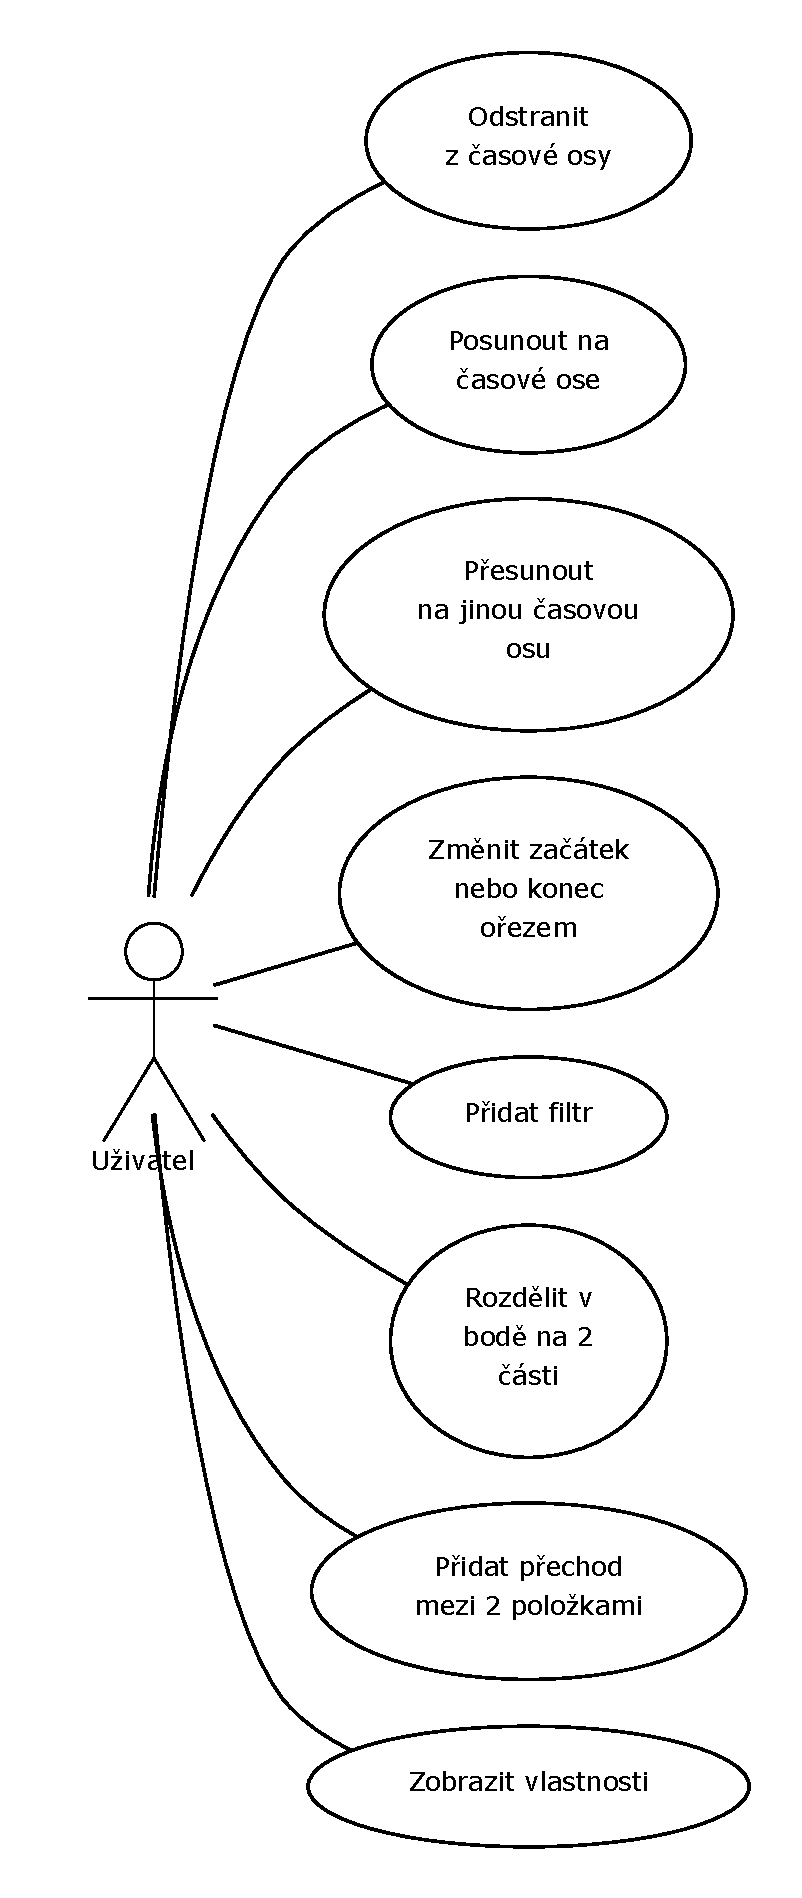
\includegraphics{obrazky-figures/ucd-polozky.pdf}
	}
	\caption{Diagram případů užití pro práci s~položkami časové osy.}\label{img:ucd-polozky}
\end{figure}

Pokud je potřeba upřesnit, jakou akci chce uživatel provést (výběr filtru), zobrazí se rozbalovací nabídka. Vyžaduje-li akce zadání hodnot, zobrazí se modální okno. Modální okna jsou využívány i pro zobrazení vlastností. Nápověda k~prvkům je řešena pomocí informačních bublin (někdy též tooltip).

Vyvedení videa (dokončení)

Pokud má nový systém nahradit stávájící proces zpracování videa, musí zvládat všechny kroky úprav videa. V~Tabulce \ref{tab:uc1} uvádím v~současnosti nejčastější případ užití, kdy je potřeba oříznout začátek a konec videa a před video vložit úvodní obrazovku s~podmínkami použití.

\begin{table}[h]
    \centering
    \begin{tabular}{|p{14cm}|}
        \hline
        Případ užití: Vložit intro, oříznout videozáznam\\ \hline
        \textbf{ID: UC1}\\ \hline
        \textbf{Účastníci:}\\
        Zaměstnanec FIT\\
        Systém\\ \hline
        \textbf{Vstupní podmínky:}\\
        1. Zaměstnanec má k~dispozici obrázek s~intro a video.\\
        2. Zaměstnanec otevřel internetové stránky s~editorem.\\ \hline
        \textbf{Tok událostí:}\\
        1. Případ užití začíná nahráním videa a obrázku intra.\\
        2. Uživatel vloží obrázek na časovou osu, v~dialogu nastaví délku zobrazení intra.\\
        3. Uživatel vloží video na časovou osu.\\
        4. Uživatel si přehraje náhled videa a v~místě plánovaného začátku a konce videa přehrávání pozastaví a provede rozdělení na 2 části.\\
        5. Uživatel zvolí část po plánovaném konci a odstraní ji.\\
        6. Uživatel zvolí část před plánovaným začátkem a odstraní ji. Ořezané video uchopí a přetáhne jej na časové ose hned za konec intra.\\
        7. Uživatel potvrdí změny a vyplní parametry výsledného videa.\\
        8. Systém generuje XML a nabízí jej ke stažení nebo zpracování na serveru.\\
        \hline
    \end{tabular}
    \caption{Textová specifikace případů užití pro nejčastější úpravy záznamů přednášek.}
    \label{tab:uc1}
\end{table}

\section{Návrh API}
Stejně jako uživatelské rozhraní i serverové rozhraní je potřeba navrhnout a otestovat. Při návrhu je třeba dbát pravidel architektury \textit{REST}. \textit{REST} definuje, jakým způsobem lze pracovat s daty na serveru. K práci se využívají 4 metody -- vytvoření dat (Create), získání požadovaných dat (Retrieve), změnu (Update) a smazání dat (Delete). Tato čtveřice bývá označování zkratkou CRUD\,\cite{rest}.

Nejprve jsem si ujasnil, jaké všechny operace bude API umožňovat. Jedná se o následující operace: vytvořit nový projekt, získat stav existujícího projektu, nahrát soubor ze zařízení, vložit nahraný soubor na časovou osu, přidat filtr, odebrat filtr, přidat přechod, odebrat přechod, posunout položku, rozdělit položku na 2 části, odebrat položku z časové osy, smazat nahraný soubor, vyvést (dokončit) projet, případně smazat projekt.

Dalším krokem bylo identifikovat zdroje -- entity. Jednou z entit bude beze sporu \textbf{projekt}, dále \textbf{soubor} a \textbf{položka časové osy}. Dalšími entitami jsem určil \textbf{přechod} a \textbf{filtr}. Operace je možné provádět jen nad zdroji, po identifikaci zdrojů je potřeba přiřadit operace ke zdrojům.

K projektu jsem přiřadil: vytvořit nový projekt, získat stav existujícího projektu, vyvést projet, smazat projekt. Nad souborem bude možné provádět: nahrát soubor ze zařízení, vložit nahraný soubor na časovou osu, smazat nahraný soubor. Položka časové osy bude umožňovat: posunout položku, rozdělit položku na 2 části, odebrat položku z časové osy. Filtr bude možné přidat a odebrat, stejně tak přechod bude možné přidat a odebrat.

\textit{REST} ovšem rozlišuje 4 metody. Nyní je potřeba přiřadit operacím jednu z následujích metod: POST (Create), GET (Retrieve), PUT (Update), DELETE (Delete). Nové prostředky vytváříme při vytváření nového projektu, nahrávání souboru ze zařízení, přidání filtru a přechodu, pro tyto operace jsem zvolil metodu POST. Získávání stavu projektu je jednoznačně metoda GET. Pro rušení prostředků slouží metoda DELETE -- odebrání filtru, odebrání přechodu, odebrání položky z časové osy, smazání nahraného souboru, smazání projektu. Na zbývající operace jsem použil metodu PUT -- vložit nahraný soubor na časovou osu, posunout položku, rozdělit položku na 2 části.

I ideálním případě nevzniknout kolize a každý zdroj bude mít přiřazenou maximálně jednu operaci k jedné HTTP metodě. V mém případě má zdroj \textbf{položka na časové ose} dvě metody PUT -- posunout položku, rozdělit položku na 2 části. V této chvíli je potřeba operace dále rozlišit, přesun identifikuji jako \texttt{move} a rozdělení položek jako \texttt{split}.

Aby nemohlo dojít ke kolizi mezi URL určených pro webové stránky a pro API, mají veškeré požadavky na API prefix \texttt{api}. Do budoucna to umožní například verzovat API. Výsledný návrh API uvádím v následujícím seznamu:
\begin{itemize}
\item project
\begin{itemize}
\item POST: \texttt{/project}
\item GET: \texttt{/project/\{projectID\}}
\item DELETE: \texttt{/project/\{projectID\}}
\item PUT: \texttt{/project/\{projectID\}}
\end{itemize}
\item file
\begin{itemize}
\item POST: \texttt{/project/\{projectID\}/file}
\item DELTE: \texttt{/project/\{projectID\}/file/\{fileID\}}
\item PUT: \texttt{/project/\{projectID\}/file/\{fileID\}}
\end{itemize}
\item filter
\begin{itemize}
\item POST: \texttt{/project/\{projectID\}/filter}
\item DELETE: \texttt{/project/\{projectID\}/filter}
\end{itemize}
\item transition
\begin{itemize}
\item POST: \texttt{/project/\{projectID\}/transition}
\item DELETE: \texttt{/project/\{projectID\}/transition}
\end{itemize}
\item item
\begin{itemize}
\item DELETE: \texttt{/project/\{projectID\}/item}
\item PUT: \texttt{/project/\{projectID\}/item/move}
\item PUT: \texttt{/project/\{projectID\}/item/split}
\end{itemize}
\end{itemize}

Požadavek na \textit{REST} API musí být úplný, \textit{REST} API je bezstavové. Například požadavek DELETE \texttt{/project/\{projectID\}} je úplný, serveru říkáme, že má smazat projekt a zároveň i uvádíme identifkátor projektu. U některých požadavků je ale potřeba blíže specifikovat parametry požadavku. Například u požadavku POST: \texttt{/project/\{projectID\}/filter} nevíme, jaký filtr se má aplikovat a ani nevíme, na jakou položku. Vyjma metody GET mohou mít požadavky tělo s parametry. Parametry mohou být předány v libovolném formátu, v projektu používám \textit{application/json} a pro nahrávání souboru \textit{multipart/form-data}. Přechozí požadavek je upřesněn parametry \texttt{track}, \texttt{item}, \texttt{filter} a \texttt{params} (parametry filtru). Kompletní specifikace navrženého API se nachází v dokumentaci API.

\chapter{Práce s multimédii}
\section{MLT framework}
Jedná se o~sadu nástrojů s~otevřeným zdrojovým kódem s~licencí LGPL-2.1, která byla původně vytvořena pro televizní vysílání. Poskytuje nástroje pro streamování, video editory, multimediální přehrávače, konvertory a další typy multimediálních aplikací. Framework MLT umožňuje vytvářet, spravovat a přehrávat audio nebo video projekty s~více stopami. Je používán jako jako základní komponenta v~nelineárních video editorech. Využití nalezne i mimo klasické desktopové video editory, může být použit jako součást většího systému nezávisle na použitém programovacím jazyce.

Framework lze používat prostřednictvím programu \texttt{melt} v~příkazovém řádku nebo prostřednictvím MLT API knihovny v~jazyce C. Pro napojení API na jiné programovací jazyky je nutné použít \textit{SWIG}\footnote{SWIG -- nástroj pro vývoj softwaru umožňující propojit program napsaný v jazyce C/C++ s jiným jazykem, \url{http://swig.org/}.}, nástroj, který překládá volání funkcí API na volání funkcí v~C++. V~C++ funkcích se následně volají funkce programu MLT v~jazyce C. Druhou možností je provádět serializaci/deserializaci dat vlastnoručně a s~MLT komunikovat prostřednictvím formátu XML. Vnitřní struktura, kterou MLT API vytváří je XML formátu blízká. V~této práci se zabývám využitím MLT XML.

\subsection{Zprovoznění}
Framework nemá žádné jiné závislosti, než standard C99 a knihovny standardu POSIX. Zprovoznění tak zahrnuje nainstalování programu \texttt{melt} (v~případě Ubuntu z~repozitáře) a nainstalovaní programů a kodeků pro práci s~multimédii.
\begin{lstlisting}[style=bash]
$ sudo apt install melt
$ sudo apt install ladspa-sdk ffmpeg
$ sudo apt install vlc #Volitelne, pro prehrani vystupu
\end{lstlisting}

\subsection{Základní příkazy}
Jednoduché úkony lze provádět volbou parametrů při spuštění programu. Pro složitější projekty bude potřeba použít serializaci dat a formát XML. Melt umí soubory XML načítat i generovat.
\begin{lstlisting}[style=bash]
#Prehrani na obrazovce
$ melt VIDEO0004.mp4 -consumer sdl
#Predpis pro vytvoreni sedotonoveho videa serializovany v XML souboru
$ melt VIDEO0004.mp4 -filter greyscale -consumer xml > task.mlt 
#Vyvedeni souboru output.avi na zaklade XML souboru
$ melt task.mlt -consumer avformat:output.avi acodec=libmp3lame vcodec=libx264
\end{lstlisting}
\subsection{Používání formátu XML}
Nejprve je nutné uvést seznam vstupních mediálních souborů. Vstupný soubor je označen jako \texttt{producer}. U~vstupu se v~\texttt{property} uvádí hodnota \texttt{resource}, s~cestou k~souboru. Tento jednoduchý soubor po spuštění přehraje celý soubor VIDEO001.mp4. Toto XML může být užitečné pokud chceme soubor pouze překonvertovat do jiného formátu.
\begin{lstlisting}[style=xml]
<?xml version="1.0"?>
<mlt>
  <producer id="producer0">
    <property name="resource">/home/vladan/VIDEO0001.mp4</property>
  </producer>
</mlt>
\end{lstlisting}
Obvykle potřebujeme pracovat s~více soubory. K~tomuto účelu slouží \texttt{playlist}. Stanovíme vstupy (\texttt{producer}) s~unikátním \texttt{id}. V tuto chvíli by se přehrál pouze poslední soubor, který uvedeme, neboť framework MLT přehraje vždy poslední element uvnitř kořenového elementu \texttt{<mlt>} . Definujeme \texttt{playlist} obsahující položky \texttt{entry}. Vstupní soubory jsou na výstup řazeny ve stejném pořadí v~jakém jsou uvedeny v~playlistu. U~položky playlistu můžeme uvést čas (od/do) pokud chceme vložit část vstupního souboru. Časové údaje-lze zadávat buď jako počet snímků nebo jako čas ve formátu \texttt{00:00:00,000}, kde první dvojice číslic jsou hodiny a poslední tři číslice udávají milisekundy. Omezení se ignoruje, pokud uvedeme větší číslo, než je počet snímků či délka souboru. Vkládáme-li obrázek, pak hodnota \texttt{out} udá délku zobrazení obrázku. S~tímto XML zvládneme sestříhat více souborů do jednoho, vystřihnout určitou pasáž, vložit intro a outro.
\begin{lstlisting}[style=xml]
<?xml version="1.0"?>
<mlt>
  <producer id="producer0">
    <property name="resource">/home/vladan/VIDEO0004.mp4</property>
  </producer>
  <producer id="producer1">
    <property name="resource">/home/vladan/VIDEO0001.mp4</property>
  </producer>
  <producer id="producer2">
    <property name="resource">/home/vladan/lego1.png</property>
  </producer>

  <playlist id="playlist0">
    <entry producer="producer2" in="0" out="50"/>
    <entry producer="producer1" in="0" out="999"/>
    <entry producer="producer0" in="0" out="100"/>
  </playlist>
</mlt>
\end{lstlisting}
Chceme-li na video aplikovat filtry, musíme vytvořit element \texttt{tractor} obsahující \texttt{multitrack} se seznamem tracků (playlistů). V~tractoru definujeme filtry. Filtry aplikujeme na \texttt{track} (playlist). Pokud budeme chtít vzít vstupní video, aplikovat na něj černobílý filtr, musíme vytvořit \texttt{playlist} s~jedním zdrojem a \texttt{tractor} s~jedním playlistem (track).
\begin{lstlisting}[style=xml]
<?xml version="1.0"?>
<mlt>
  <producer id="producer0">
    <property name="resource">/home/vladan/VIDEO0002.mp4</property>
  </producer>
  <tractor id="tractor0">
    <multitrack>
      <playlist id="playlist0">
        <entry producer="producer0"/>
      </playlist>
    </multitrack>
    <filter mlt_service="greyscale" track="0"/>
  </tractor>
</mlt>
\end{lstlisting}
Pokud potřebujeme aplikovat filtr na část videa, musíme vytvořit dva playlisty -- jeden pro část na kterou bude aplikován filtr a druhý playlist pro část bez filtru. Pro synchronizaci playlistů použijeme \texttt{blank}, v~jednu chvíli se může zobrazovat pouze jeden z~playlistů, přednost má ten později zadefinovaný. V~následujícím případě se v~playlist1 prvních 100 snímků přehrává VIDEO0002, v~playlist2 je po tuto dobu nastaven stav \texttt{blank}. Pokud chceme zobrazovat statickou překryvnou vrstvu, můžeme využít filtru \texttt{watermark}. Pokud je filtr přizpůsobitelný parametry, uvedou se uvnitř elementu \texttt{filter} stejným způsobem, jako se uvádí parametry u elementů \texttt{producer}.
\begin{lstlisting}[style=xml]
<?xml version="1.0"?>
<mlt>
  <producer id="producer0">
    <property name="resource">/home/vladan/VIDEO0002.mp4</property>
  </producer>
  <tractor id="tractor0">
    <multitrack>
      <playlist id="playlist0">
        <entry producer="producer0" in="0" out="99"/>
        <blank length="50"/>
        <entry producer="producer0" in="150"/>
      </playlist>
      <playlist id="playlist1">
        <blank length="100"/>
        <entry producer="producer0" in="100" out="149"/>
      </playlist>
    </multitrack>
    <filter mlt_service="watermark" track="0">
      <property name="resource">transparent.png</property>
    </filter>
    <filter mlt_service="greyscale" track="1"/>
  </tractor>
</mlt>
\end{lstlisting}
Více stop (\texttt{track}) může být přehráváno současně pouze použijeme-li filtr nebo přechod. Přechody (\texttt{transition}) se aplikují stejně jako filtry uvnitř tractoru. U~přechodu nastavíme snímek náběhu a dokončení přechodu (\texttt{in} a \texttt{out}) a dále specifikujeme typ přechodu (\texttt{mlt\_service}) dle \url{https://www.mltframework.org/plugins/PluginsTransitions/}, počáteční stopu přechodu (\texttt{a\_track}) a cílovou stopu přechodu (\texttt{b\_track}). Tímto způsobem můžeme vytvořit intro nebo outro s~přechody, či prolínání jednotlivých video souborů. Obě stopy by se měly překrývat pouze po dobu přechodu. Pokud by například přechod skončil dříve, než by začala druhá stopa, docházelo by ke krátkodobému probliknutí první stopy.
\begin{lstlisting}[style=xml]
<mlt>
  <producer id="producer0">
    <property name="resource">lego1.png</property>
  </producer>
  <producer id="producer1">
    <property name="resource">VIDEO0001.mp4</property>
  </producer>
  <tractor id="tractor0">
    <multitrack id="multitrack0">
      <playlist id="playlist0">
        <entry producer="producer0" in="0" out="74"/>
      </playlist>
      <playlist id="playlist1">
        <blank length="50"/>
        <entry producer="producer1"/>
      </playlist>
    </multitrack>
    <transition mlt_service="luma" in="50" out="74" a_track="0" b_track="1"/>
  </tractor>
</mlt>
\end{lstlisting}

S~pomocí těchto konstrukcí jsme schopni nadefinovat nejčastější operace, které se při zpracovávání přednášek provádí.

\section{Práce s videi v prohlížeči}
S příchodem HTML5 prvků \texttt{<video>} a \texttt{<audio>} a jejich JavaScriptového API vzniká možnost práce s multimédií na webu. Práci s multimediálními prvky implementovali od roku 2010 všechny moderní prohlížeče. Za moderní desktopové prohlížeče považuji program Google Chrome, Safari, Mozilla Firefox, Opera, Microsoft Edge. Prohlížeč Internet Explorer má sice dle serveru StatCounter 5.48\% zastoupení, což jej řadí mezi Microsoft Edge a Operu\,\cite{statcounter}, avšak i Microsoft jej v únoru označil za \uv{řešení pro kompatibilitu}, nikoliv webový prohlížeč\,\cite{internetExplorer}. Po představení prohlížeče Microsoft Edge získává Internet Explorer bezpečnostní záplaty, ale neprobíhá implementace nových webových standardů. Při vývoji nových projektů by tedy nekompatibilita s Internet Explorer neměla být brána v potaz. Následující kapitoly čerpají z knihy \textit{HTML5 - audio a video: kompletní průvodce}\,\cite{HTML5multimedia} a z komunitního projektu MDN Web Docs\footnote{MDN Web Docs -- portál s webovou dokumentací provozovaný společností Mozilla, \url{https://developer.mozilla.org/}}.

\subsection{Kódování mediálních zdrojů}
Veškerá data v počítači je potřeba kódovat. Na vyšší úrovni pohlížíme na kódování jako na formát dat. Formáty kódování audia  jsou například MP3, AAC, Vorbis, FLAC a formáty kódování videa například MPEG-2, MPEG-4 , H.264, HEVC, Theora, VP9, AV1.  Z pohledu uživatele se liší zejména licencí pro použití a způsobem komprese dat. Multimediální soubory mohou obsahovat více video a audio stop, titulky či jiná podpůrná data, proto se multimediální soubory vždy obalují do multimediálních kontejnerů, jako například AVI, MP4, FLV, RealMedia, Matroška. Výběr formátu videa tak typicky zahrnuje výběr multimediálního kontejneru, formátu kódování videa a formátu kódování audia. Kodek je zařízení nebo počítačový program, který dokáže převádět zakódovaná data do jiné podoby, v případě webových aplikací je kodekem internetový prohlížeč. V době, kdy organizace W3C\footnote{World Wide Web Consortium (W3C) -- mezinárodní sdružení vytvářející webové standardy, \url{https://www.w3.org/}.} vytvářela specifikaci pro HTML5 prvky \texttt{<video>} a \texttt{<audio>} byla snaha standardizovat formát, který by byl podporován ve všech prohlížečích neúspěšná kvůli požadavku na royalty free licenci\,\cite{HTML5multimedia}. Od té doby se nejvíce rozšířil formát MP4 H.264, který ovšem odmítá Mozilla a Theora, který odmítá Apple. Pokud se podíváme dnes na srovnání podporovaných kodeků, tabulka \ref{tab:codecs}, zjistíme, že situace není jednoduchá.
\begin{table}[h]
    \centering
    \begin{tabular}{|l|l|l||l|l|l|l|l|}
    \hline
    Kontejner   & Video & Audio & Chrome & Firefox & Edge & Opera & Safari \\
    \hline
    WebM        & VP8   & Vorbis &ano & ano & s 2 rozšířeními & ano & ne* \\
    WebM        & VP9   & Opus & ano & ano & rozšíření, HW dekodér & ano & ne \\
    WebM        & AV1   & Vorbis & ano & ano & s beta rozšířením & ano & ne \\
    WebM        & AV1   & Opus & ano & ano & s beta rozšířením & ano & ne \\
    Ogg         & Theora & Vorbis & ano & ano & s rozšířením & ano & ne \\
    MP4         & H.264 & MP3 & ano*** & ano** & ano & ano & ano \\
    MP4         & H.264 & AAC & ano*** & ano** & ano & ano & ano \\
    \hline
    \end{tabular}
    \caption{Přehled široce podporovaných formátů videa internetovými prohlížeči.}
    \label{tab:codecs}
\end{table}\\
* Safari vyžaduje pro VP8 program Perian\footnote{Perian -- program pro MacOS rozšiřující podporu QuickTime o další formáty (vývoj ukončen) ,\url{https://www.perian.org/}.}.\\
** Mozilla Firefox pro Linux vyžaduje pro H.264 program GStreamer\footnote{GStreamer -- otevřený multiplatformní multimediální framework, \url{https://gstreamer.freedesktop.org/}.} nebo FFmpeg.\\
*** Google Chrome H.264 podporuje, ale Chromium vyžaduje FFmpeg.
\medskip

Pokud bychom chěli použít pouze jeden formát, můžeme zvolit H.264 video s AAC audiem uvnitř MP4 nebo VP8 video s Vorbis audiem uvnitř WebM. V prvním případě budou muset uživatelé prohlížeče Firefox na Linuxových systémech a uživatelé prohlížeče Chromium nainstalovat program FFmpeg, v druhém případě budou muset užiatelé Safari nainstalovat program Perian a uživatelé Microsoft Edge Rožšíření pro webová média a Rozšíření pro video VP9.

Chceme-li mít jistotu, že uživatel video přehraje, pak musíme zvolit formáty dva -- H.264 s MP3/AAC uvnitř MP4 pro uživatele Safari a Edge a pro ostatní uživatele variantu Theora s Vorbis uvnitř Ogg.

\subsection{Použití prvku video}
Prvek \texttt{<video>} přinesla specifikace HTML5 a umožňuje přehrávat video na webové stránce v režii prohlížeče. Pokud nespecifikujeme jinak, prohlížeč zajistí načtení zdroje a vykreslení ovládacích prvků. S videem můžeme pracovat skrze atributy a HTMLMediaElement API. Prvek je podporován všemi rozšířenými prohlížeči s výjimkou Opera Mini (kvůli spořiči přenesených dat).

Video prvek má celkem 6 atributů. Atributy \texttt{autoplay}, \texttt{loop} a \texttt{controls} mohou nabývat booleovských hodnot a proto jejich uvedení znamená logickou 1, pokud atributy neuvedeme, jsou atributy s hodnotou logické 0. Pro potřeby náhledu videa atribut \texttt{autoplay} nepoužijeme, video budeme přehrávat skrze API metody \texttt{play}, \texttt{loop} rovněž není žádoucí, video by se přehrávalo ve smyčce, při neuvedení se přehrávání na konci zastaví. Atribut \texttt{controls} zobrazí ovládací prvky, což je nežádoucí, použijeme vlastní ovládací prvky. Atribut \texttt{preload} navrhuje prohlížeči, kolik dat se má načíst ze zdroje, dostupné hodnoty jsou \uv{none}, \uv{metadata} a \uv{auto}. Hodnota \uv{none} nenačte nic, \uv{metadata} zajistí načtení délky videa a prvního snímku, \uv{auto} nechá volbu na prohlížeči. V případě editoru postačuje výchozí hodnota \uv{auto}. Atribut \texttt{poster} slouží k nahrazení prvního snímku zástupným obrázkem, v projektu není potřebný. Praktické jsou elementy \texttt{width} a \texttt{height}, udávají šířku a výšku videa. Rozměry jsou chápány jako maximální možné, pokud je rozměr videa větší, zmenší se ve výchozím nastavení se zachováním poměru stran. Zarovnání videa v boxu určuje CSS vlastnost \texttt{boject-position} s dvojicí hodnot pro vodorovnou a svislou pozici. Jak se má měnit měřítko obsahu videa vlastnost \texttt{object-fit} s hodnotami \uv{fill}, \uv{contain} a \uv{cover}.

Zdroj videa lze nastavit dvěma způsoby. Atributem \texttt{src} nebo vnořenými prvky \texttt{<source>}. Vnořené prvky \texttt{<source>} poskytují více možností skrze vlastní atributy. Zdrojů můžeme uvést více s různými formáty -- atribut \texttt{type} (MIME typ mediální zdroje) nebo \texttt{media} (mediální zdroj pro konkrétní typ zařízení). Prohlížeč sám vybere pro něj nejlepší zdroj. Pokud měníme zdroje dodatečně, musíme po změně zavolat metodu \texttt{load}, která provede inicializaci video prvku. Druhou možností je uvést zdroj v atributu \text{src} prvku \text{<video>}. Takto je možné nastavit jen jeden zdroj současně, a proto si musíme kompatibilitu formátu sami skrze metodu \texttt{canPlayType} nebo knihovny Modernizer\footnote{Modernizer -- sada nástrojů pro testování funkcí prohlížeče, \url{https://modernizr.com/}.}. Druhá metoda je vhodná pokud používáme jeden zdroj.

\subsection{Použití prvku audio}
Prvek pro přehrávání audia v prohlížeči je možné rovněž upravovat pomocí HTMLMediaElement API a pomocí atributů. Prvek \texttt{<audio>} narozdíl od videa nemá atributy \texttt{poster}, \texttt{width}, \texttt{height}, protože jsou v prohlížeči vykresleny pouze ovládací prvky bez vizualizace audia. Audio prvek lze využít pro zvukové stopy. Nastavení a význam hodnot atributů je stený jako u prvku \texttt{<video>}.

\subsection{Ovládání videa}
Přehrávání videa lze ovládat pomocí JavaScriptu skrze HTMLMediaElement API. Stejné API používají i prvky \texttt{<audio>}, lze pro ně použít stejný postup. Základními metodami pro přehrávání jsou \texttt{play} a \texttt{pause}. Přehrávání videa se na konci zastaví (pokud není nastaven atribut \texttt{loop}). Pokud po dokončení přehrávání zavoláme znovu metodu \texttt{play}, přehrávání se spustí od začátku videa.

Pro skok na konkrétní pozici slouží atribut \texttt{currentTime}. Atribut je určen pro čtení (získání aktuálního času) i pro zápis (skok na pozici). Celkovou délku zjistíme přečtením atributu \texttt{duration}. Délku musíme zjišťovat až po získání metadat -- odpálení události \texttt{loadedmetadata}.

Další užitečnou událostí je \texttt{timeupdate}, která se volá v intervalech 15 ms až 250 ms (Mozilla Firefox 100-250 ms) po čas přehrávání a umožňuje průběžně efektivně pracovat s atributem \texttt{currentTime} a například zobrazovat aktuální pozici přehrávání.

Použití událostí a metod pro jednoduchý přehrávač videa řízený JavaScriptem ukazuje obrázek \ref{img:html-control}.

\begin{figure}[h]
	\centering
	\scalebox{0.7}{
		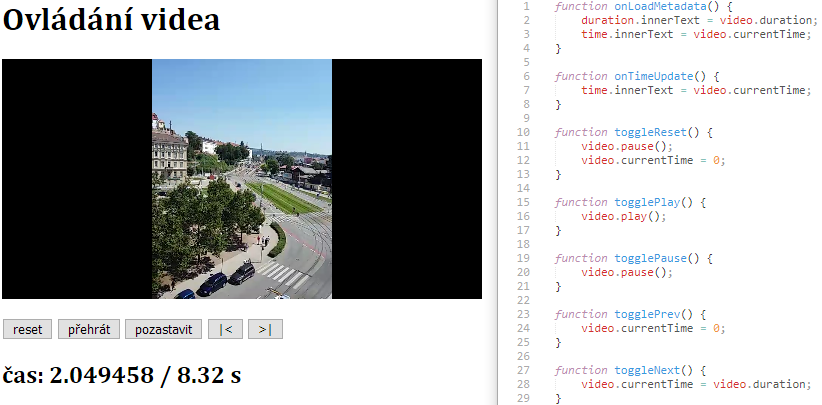
\includegraphics{obrazky-figures/html-control.png}
	}
	\caption{Jednoduchý přehrávač videa demonstrující využití HTMLMediaElement API.}\label{img:html-control}
\end{figure}

\subsection{Posloupnost videí}
Při dosažení konce média je odpálena událost \texttt{ended}. Této události lze využít pro vytváření posloupnosti videí. Plocha s náhledem je tvořena dvojicí videí. Na popředí je aktuálně přehrávající se videa a na pozadí je skryté druhé video, které se s předstihem nastaví na nový zdroj, počáteční pozici a načtou se metadata. Jakmile přehrávání videa v popředí skončí a je odpálena událost \texttt{ended}, dojde k prohození videa v popředí s videem v pozadí a spustí se nové video v popředí. Přístup dvou scén, kdy jedna je viditelná a druhá se připravuje, je inspirován programem OBS Studio\footnote{OBS Studio -- open source software pro nahrávání a streamování videí, \url{https://obsproject.com/}.}, který slouží na nahrávání a streamování videí. Ve webovém prohlížeči určuje pořadí objektů CSS vlastnost \texttt{z-index}. Hodnotou je celé číslo, objekty s vyšší hodnotou překryjí objekty s nižší hodnotou. Prvky se musejí překrývat, to lze zajistit absolutním pozicování uvnitř obalovacího kontejneru. Následující kód obsahuje funkci pro přehození video souborů a pro resetování přehrávače do původního stavu.
\begin{lstlisting}[style=JavaScript]
let videoMain = video1;
function videoSwap() {
    videoMain = video2;
    video1.style.zIndex = 1;
    video2.style.zIndex = 2;
    togglePlay();
}

function toggleReset() {
    videoMain.pause();
    video1.currentTime = 0;
    video2.currentTime = 0;
    video1.style.zIndex = 2;
    video2.style.zIndex = 1;
    videoMain = video1;
}
\end{lstlisting}
Pro posloupnost více videí je zapotřebí \uv{podavač} videí, který přehrávači předá další klip.

\subsection{Přechod mezi videi}
Při stříhání videí se může hodit efekt prolnutí mezi 2 klipy. Při tomto přechodu se určitý čas před koncem přehrávaného videa začne přehrávat i video následující a současné video se postupně zprůhlední. Průhlednost elementů lze nastavit CSS stylem \texttt{opacity}, přičemž hodnota 1 značí neprůhledný objekt a hodnota 0 zcela průhledný objekt. Samotné prolnutí (zvyšování průhlednosti) lze provést CSS animacemi nebo snižováním hodnoty \texttt{opacity} s každým odpálením události \texttt{timeupdate}. Použití animací sice vytvoří plynulý efekt, ale nastává problém při pozastavení a obnovení videa v místě přechodu, neboť by animace musela být pozastavena, aktuální stav uložen a posléze vytvořena nová animace pro zbývající úsek. Řešení pomocí \texttt{timeupdate} poskytuje pro náhled dostatečnou kvalitu a provést pozastavení či skok je v tomto případě snadné. Pokud chceme aplikovat prolnutí, stačí nastavit délku přechodu a poté zaregistrovat následující funkci pro obsluhu události \texttt{timeupdate}.
\begin{lstlisting}[style=JavaScript]
videoMain.addEventListener('timeupdate', transitionLuma, false);
function transitionLuma() {
    const timeToEnd = videoMain.duration - videoMain.currentTime;
    if (timeToEnd <= transitionDuration) {
        videoMain.style.opacity = (timeToEnd / transitionDuration);
        if (!transition) {
            videoBack.play();
            transition = true;
        }
    }
}
\end{lstlisting}
Na každou událost lze zaregistrovat více obslužných funkcí, po skončení přechodu je nutné obsluhu funkcí \texttt{transitionLuma} odregistrovat. Pokud je zbývající čas menší nebo roven délce přechodu, nastaví se \texttt{opacity} na hodnotu rovnou podílu zbývajícího času s délkou přechodu (klesá rovnoměrně od 1 k 0). Ve webovém prohlížeči lze sestrojit i jiné přechody s odsunutím, zvětšováním, postupným odkrýváním, ale tyto filtry nejsou pro tvorbu přednášek vhodné a proto je není potřeba implementovat.

Stejnou technikou se sestrojí roztmívání a zatmívání obrazu (přechod z černé / do černé), pouze bude druhá scéna až za podkladovou černou vrstvou (\texttt{z-index se zápornou hodnotou}).

\subsection{Filtry}
Pokud potřebujeme aplikovat filtr obrazu, nabízí se dvě možnosti -- řešení pomocí CSS filtrů a řešení pomocí vykreslování do Canvas. Obě varianty mají své přednosti, CSS najde uplatnění u jednoduchých filtrů, vykreslování do Canvas nám dá absolutní kontrolu nad výsledným videem.

\subsubsection{Obrazové filtry pomocí CSS}
HTML5 obsahuje pracovní návrh CSS vlastnosti \texttt{filter}. Vlastnost aplikuje grafické efekty na libovolné objekty, včetně obrázků a video elementů. CSS vlastnost má několik definovaných filtrů a možnost odkazovat na SVG filtry. Ačkoliv se jedná o pracovní návrh, CSS filtry jsou podporovány všemi rozšířenými prohlížeči (Internet Explorer je nepodporuje).\footnote{CITACE cssFilter \url{https://developer.mozilla.org/en-US/docs/Web/CSS/filter}} Microsoft Edge podporuje předdefinované filtry, ale kvůli chybě nepodporuje odkazování na SVG filtry. Největší předností CSS filtrů je způsob aplikování na video. Filtr je uložen v CSS třídě, případně lze přiřadit přímo k elementu. U \texttt{<video>} elementu stačí nastavit třídu filtru a filtr se aplikuje, vykreslování zajistí prohlížeč. Jaké předdefinované filtry vlastnost \text{filter} nabízí, ukazuje tabulka \ref{tab:filters}.
\begin{table}[h]
    \centering
    \begin{tabular}{|l|l|l|l|l|l|l|l|}
    \hline
    Funkce filtru   & Výchozí & Možné hodnoty & Chování filtru \\
    \hline
    \textbf{brightness}  & 1 & >=0\% / >=0 & 0\% černý obraz, >100\% větší jas \\
    \textbf{contrast}    & 1 & >=0\% / >=0 & 0\% šedý obraz, >100\% větší kontrast\\
    \textbf{saturate}    & 1 & >=0\% / >=0 & 0\% vybledlý, >100\% větší sytost\\
    grayscale   & 0 & 0\%-100\% / 0-1 & 0\% původní obraz, 100\% šedotónový\\
    invert      & 0 & 0\%-100\% / 0-1 & 0\% původní obraz, 100\% invertovaný\\
    sepia       & 0 & 0\%-100\% / 0-1 & 0\% původní obraz, 100\% sépiový\\
    opacity     & 1 & 0\%-100\% / 0-1 & 0\% průhledný, 100\% neprůhledný\\
    hue-rotate  & 0 & úhel (deg/grad/rad/turn) & posun barev (s periodou 360$^{\circ}$)\\
    blur        & 0 & vzdálenost, vyjma \% & rozmazání o danou vzdálenost \\
    drop-shadow & none & viz vlastnost \texttt{box-shadow} & efekt zrcadlení\\
    \hline
    \end{tabular}
    \caption{Seznam definovaných filtrů. Klíčovými filtry jsou jas, kontrast a sytost.}
    \label{tab:filters}
\end{table}\\

Poslední možnou hodnotou, které může \texttt{filter}, je \text{url()}. V tomto případě se nejedná o filtr, ale o odkaz na SVG element. SVG element se používá jako kontejner pro SVG filtry. SVG filtry jsou z pohledu standardu ve stavu \uv{doporučení}. Aktuálně kvůli chybě nefungují v prohlížeči Mirosoft Edge. Po aplikování filtrů bylo patrné snížení počtu snímků za sekundu, při aplikování jednoho filtru bylo přehrávání videa dostatečně plynulé. Pokud bychom chtěli aplikovat více obrazových filtrů současně (4 a více), vyplatí se realizovat filtry pomocí Canvas. K dispozici je 17 filtrů, jejich přehled uvádím v tabulce \ref{tab:svg}

\begin{table}[h]
    \centering
    \begin{tabular}{|l|l|l|l|l|l|l|l|}
    \hline
    Filtr   & Popis & Možné použití \\
    \hline
    feBlend & míchání barev objektů/bitmap & přidání vodoznaku \\
    feColorMatrix & změna barev pixelů tranformační maticí & barevný odstín, sytost \\
    feComponentTransfer & úprava barevných složek & jas, kontrast \\
    feConvolveMatrix & aplikování konvoluční matice na obraz & rozmazání, doostření \\
    feGaussianBlur & Gaussovské rozmazání obrazu & rozmazání \\
    feComposite & operace nad skládáním SVG objektů & \\
    feDiffuseLighting & aplikace difúzní složky osvětlovacího modelu & \\
    feDisplacementMap & nahrazení pixelů pixely z jiného zdroje & \\
    feDropShadow & vytvoření efektu stínu/zrcadlení & \\
    feFlood & vyplění objektu konstantní barvou & \\
    feImage & převádí externí zdroj na bitmapu & \\
    feMerge & aplikuje filtry současně, ne postupně & \\
    feMorphology & zvýšení/snížení tloušťky objektů & \\
    feOffset & posun objektů v ose x, y & \\
    feSpecularLighting & aplikace lesklé složky osvětlovacího modelu & \\
    feTile & vyplnění objektu texturou & \\
    feTurbulence & generování textury pomocí Perlinova šumu & \\

    \hline
    \end{tabular}
    \caption{Seznam SVG filtrů s možným využitím ve videoeditoru.}
    \label{tab:svg}
\end{table}
Pro potřeby úprav videí nevyužijeme zdaleka všechny funkce, lze se tedy omezit na předdefinované filtry, které fungují i v prohlížeči Microsoft Edge. JavaScript umožňuje výpočetní operace nad daty pro zvýšení výkonu přesunout na pozadí do samostatného vlákna, pro tuto techniku se používá termín Web Workers.\footnote{Web Workers -- standardizované API pro běh skriptů na pozadí, \url{https://developer.mozilla.org/en-US/docs/Web/API/Web_Workers_API/Using_web_workers}.} Přímo v prohlížeči můžeme například analyzovat obsah videa a detekovat v něm objekty (například rozpoznání obličeje). Vytváření vláken přináší režii, která se vyplatí až při náročných skriptech, aplikování filtrů na videa pomocí Web Workers počet zpracovaných snímků za sekundu zvýší minimálně, ve většině prohlížečů spíše způsobí snížení (v závislosti na implementaci Web Workers). 

\subsubsection{Obrazové filtry pomocí Canvas}
Zatímco CSS a SVG filtry umožňují manipulovat s výsledným obrazem na základě přiřazení CSS stylů a tříd, Canvas přestavuje kreslící plátno složené z 2D matice pixelů. Jedná se o bitmapu, jejíž vykreslení musíme sami zajistit. Vykreslováním do canvasu lze dosáhnout větší počtu vykreslených snímků za sekundu, než při použití CSS/SVG filtrů. Canvas je vhodné použít vždy, pokud nepotřebujeme přístup k objektům filtrů pomocí DOM. Rychlost vykreslení závisí na velikosti plátna. Při velkém formátu je výhodnější SVG, než canvas. Obě techniky je možné kombinovat.

Pro zobrazení videa skrze \texttt{<canvas>} bude zapotřebí jak \texttt{<canvas>}, tak i \texttt{<video>} element. Z video elementu se budou vzorkovat snímky a vykreslovat jako bitmapy v \texttt{<canvas>}. Ovládání videa bude stále skrze JavaScriptové API \texttt{<video>} elementu, ale zobrazení obstará \texttt{<canvas>}. Z toho důvodu je nutné video element skrýt pomocí CSS vlastnosti \texttt{display: none}.

Během přehrávání je potřeba zajistit pravidelné překreslování Canvasu. Lze použít události \texttt{timeupdate}, ale tato událost je odpálena jen každých 15 ms až 250 ms, což na pohodlné přehrávání nestačí. Druhou možností je nastavit obsluhu události \texttt{play} na funkci, která bude zajišťovat překreslování. Na konci funkce pro překreslení  se otestuje, zda-li se video stále přehrává (\texttt{video.paused || video.ended}) a případně se naplánuje opětovné zavolání funkce za 0 milisekund -- \texttt{setTimeout(repaint, 0)}. V některých prohlížečích se funkce \texttt{timeupdate} neodpálí po načtení metadat a prvního snímku, pro tyto prohlížeče pomůže funkci vykreslení zavolat i pro \texttt{loadedmetadata}. Následující ukázka získá aktuální snímek z \texttt{<video>} elementu, tyto data si zkopíruje do pomocného pole a poté postupně projde a modifikuje jednotlivé pixely (v tomto případě sníží jas na polovinu). Pole pixelů je organizováno po řádcích, přičemž každý pixel se skládá ze 4 po sobě jdoucích složek (RGBA) -- každý pixel má v poli velikost 4. Po modifikaci pixelů dojde k vyčištění původního plátna (nastaví průhledné plátno) a poté vykreslý modifikovaný obraz. Pokud se video stále přehrává, naplánuje ihned další spuštění funkce \texttt{painFrame}.
\begin{lstlisting}[style=JavaScript]
video.addEventListener('play', paintFrame, false);
const context = canvas.getContext('2d');

function paintFrame() {
    context.drawImage(video, 0, 0, 480, 270, 0, 0, 480, 270);
    const frame = context.getImageData(0, 0, 480, 270);
    const output = context.createImageData(480, 270);
    
    for (let x = 0; x < 480; x++) {
        for (let y = 0; y < 270; y++) {
            let index = 4 * (x + 480 * y);
            output.data[index + 0] = frame.data[index + 0] / 2; // R
            output.data[index + 1] = frame.data[index + 1] / 2; // G
            output.data[index + 2] = frame.data[index + 2] / 2; // B
            output.data[index + 3] = frame.data[index + 3]; // A
        }
    }
    context.clearRect(0, 0, 480, 270);
    context.putImageData(output, 0, 0);
    if (!video.paused && !video.ended) {
        setTimeout(paintFrame, 0);
    }
}
\end{lstlisting}

V ukázce není vyřešeno škálování. Metoda \texttt{drawImage} vezme originální obraz, nikoliv zmenšený obraz \texttt{<video>} elementu. Pro bezpečné použití by bylo zapotřebí zjišťovat větší rozměr videa a ten přizpůsobit velikosti plátna. Dále by muselo být video ručně centrováno. V prohlížeči Mozilla Firefox se videa natáčená na výšku zobrazují v \texttt{<canvas>} otočená o 90$^{\circ}$. Z tohoto důvodu jsem od filtrů pomocí Canvas opustil.

Canvas najde uplatnění zejména v případech, kdy pracujeme s důvěryhodnými daty a provádíme nad nimi náročné operace. 

\subsection{Shrnutí}
HTML5 je živý standard, který neustále rozšiřuje možnosti tvorby webového obsahu. Práce s multimédii je v HTML5 prakticky neomezená, ale ne všechny funkce jsou standardizovány. Při implementaci je nutné sledovat stav standardu a rozšířenost v prohlížečích. Vždy je nutné začít výběrem formátu multimédií. Pokud chceme mít jistotu, že každý uživatel bude mít prohlížeč s kompatibilním kodekem, musíme prohlížeči videa nabízet alespoň ve 2 formátech. Jednoduché úpravy obrazu provádíme pomocí CSS filtrů, na složitější filtry použijeme SVG filtry. Chceme-li přistupovat přímo k obrazovým datům, použijeme Canvas. Jednoduchý videoeditor si pro náhledové video vystačí s CSS filtry -- dostatečně rychlé, na implementaci jednoduché a s podporou v moderních prohlížečích.

\chapter{Realizace, experimenty}

\section{Generování XML}
Se založením nového projektu je vytvořen soubor \texttt{project.mlt} obsahující hlavičku XML a odkaz na DTD schéma umístěné v repositáři projektu MLT. Poté následuje kořenový tag \texttt{<mlt>}. Uvnitř se nachází jeden playlist pro výchozí stopu \texttt{videotrack0} a hlavní kontejner \texttt{<track>} obsahující odkazy na všechny stopy v projektu. Tento hlavní kontejner musí být vždy poslední položkou v kořenovém \texttt{<mlt>}.

Uvnitř kořenového elementu se nejprve  nacházejí zdrojové soubory (elementy <producer>) u kterých jsou poznamenány následující vlastnosti -- absolutní cesta k souboru (\texttt{resource}), typ souboru (\texttt{musecut:mime\_type}), původní název souboru (\texttt{musecut:name}) a v případě video souboru délka v milisekundách (\texttt{length}). Zdrojové soubory mají id s prefixem \uv{producer} a 20 znaky náhodně generovanými při nahrávání souboru.
Po posledním elementu \texttt{<producer>} jsou pomocné playlisty
\begin{figure}[h]
	\centering
	\scalebox{0.6}{
		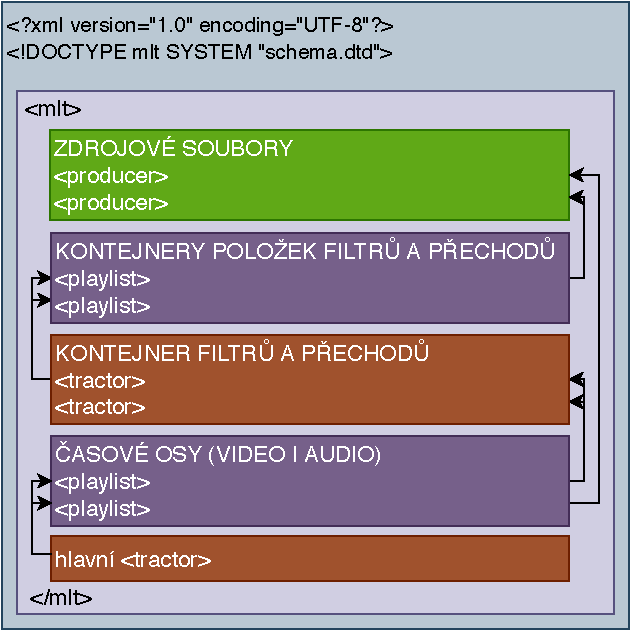
\includegraphics{obrazky-figures/schemaXML.pdf}
	}
	\caption{Obecné schéma prvků generovaných souborů.}\label{img:schemaXML}
\end{figure}


\section{API serveru}
\section{Zvolené technologie}
\begin{itemize}
\item Google Material Icons -- \url{https://github.com/jossef/material-design-icons-iconfont}
\item Visual timeline -- vis.js \url{https://github.com/almende/vis}
\item FFMPEG JS API: \url{https://github.com/bilashcse/Online-Video-Editor}
\item FFmpeg v~JavaScriptu: \url{https://github.com/bgrins/videoconverter.js}
\item Python knihovna pro usnadnění práce s~MLT frameworkem: \url{https://github.com/antiboredom/vidpy}
\end{itemize}
Emaily:
\begin{itemize}
\item odesílání \texttt{nodemailer}
\item zachytávání pro testování \texttt{Papercut} / \texttt{smtp-sink} (node.js řešení)
\end{itemize}

Volba PHP vs Node.js. Volba EcmaScript vs TypeScript vs CoffeeScript.
\begin{figure}[h]
	\centering
	\scalebox{0.4}{
		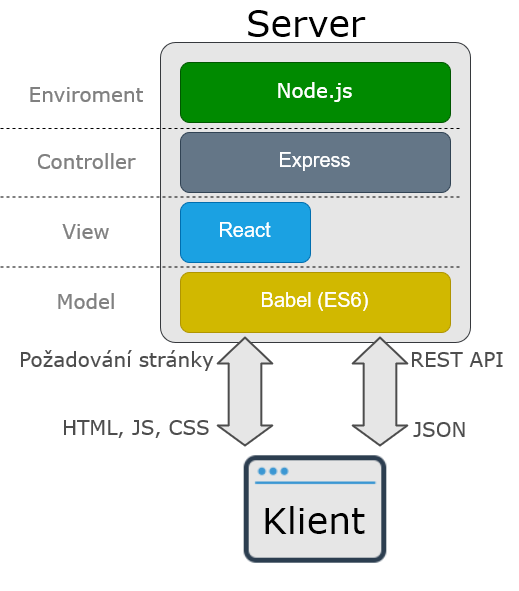
\includegraphics{obrazky-figures/server-architektura.png}
	}
	\caption{Architera serveru.}\label{img:server-architektura}
\end{figure}

\subsection{Node.js}
Node.js vytváří běhové prostředí JavaScriptu postavené na JavaScriptovém enginu V8 od firmy Google. Umožňuje používat JavaScript jako systémový jazyk, který má přístup k paměťi, bufferům, procesům, souborům a soketům. Cílem Node.js je poskytovat snadnou cestu k vytvoření škálovatelných síťových aplikací. Node.js nepoužívá vlákna, je založen na událostech a asynchronním vykonávání blokujících operací, umožňuje snadnou modularitu. Právě eliminací blokujících operací pomocí asynchronní obsluhy řízenou událostmi lze dosáhnout vysokého výkonu. PHP vytváří pro každý požadavek samostatné vlákno a v případě blokující operace čeká na vyřízení, Node.js používá pro všechny požadavky jedno vlákno a namísto paralelního zpracování používá Node.js pseudoparalelní zpracování.

Pro porovnání rychlosti vykonání programu, uvedu příklad jednoduchého programu, ve kterém se v prázdném cyklu inkrementuje miliadkrát čítač. Doba běhu programu je pro jednotlivé jazyky následující -- JavaScript (Node.js verze 9.3.0) 0,635 sekund, jazyk C (Apple LLVM 8.1.0) 2,398 sekund a Python (3.6.1) 31,096 sekund. Všechny testy probíhaly na zařízení MacBook Pro s procesorem Intel Core i7 2,8 GHz. Překladač V8 JavaScript kompiluje namísto interpretování, díky tomu lze využívat vysokoúrovňový jazyk bez nutnosti vzdát se rychlosti kompilovaných jazyků\,\cite{MasteringNodejs}.

JavaScript na klientské straně je pro interaktivní webovou aplikaci nutnost. Díky běhu JavaScriptu na klientské i serverové části mohou programátoři používat jeden jazyk v rámci projektu. Dále se otevírá možnost používat stejný kód na serveru i na straně klienta. Stačí vhodně členit funkce do modulů a tyto moduly poté importovat jak na straně serveru, tak na straně klienta. V mé práci takto sdílím kód pro práci s časovými značkami.

\subsubsection{Souborový systém}
Práci se souborovým systémem umožňuje modul File System (\texttt{fs}). Používání funkcí modulu \texttt{fs} je podobné POSIX funkcím jazyka C. Všechny funkce mají synchronní a asynchronní variantu. U I/O operací je silně doporučeno používat asynchronní práci se souborovým systémem. Asynchronní funkce mají jako poslední parametr callback, který se zavolá po dokončení operace. Callbacku je jako první parametr předán objekt pro uchování chyb a poté volitelně data operace. Callback je volán při úspěchu i neúspěchu, neúspěch je indikován objektem 1. parametru. Dalším modulem spojeným se souborovým systémem je \texttt{path}, který poskytuje nástroje pro práci s cestami k souborům a adresářům. Jak vypadá asynchronní čtení souboru ukazuje následující ukázka.
\begin{lstlisting}[style=JavaScript]
fs.open(path.join(projectPath, 'processing')), 'wx', (err, fd) => {
    if (err) throw err;
    // prace se souborem
    fs.close(fd, (err) => {
        if (err) console.error(err.stack);
    };
});
console.log('stale se muze cekat na nacteni souboru);
\end{lstlisting}

Funkce \texttt{fs.open} je zavolána, vytvoří požadavek souborovému systému a namísto aktivního čekání je funkce uspána a pokračuje se dál vykonáváním příkazů pod \texttt{fs.open}. V tomto případě by se vypsal do terminálu text \uv{stale se muze cekat na nacteni souboru} a k práci se souborem by se JavaScriptový engine vrátil až po zpřístupnění požadovaného souboru. Z toho plyne, že I/O operace jednoho požadavku nebrzdí vykonávání souběžných požadavků.

\subsubsection{Práce s procesy}
Díky událostem a asynchronnímu přístupu k blokujícím požadavkům není problém čekat na mnohem náročnější operace, než je práce se souborovým systémem. V projektu je potřeba zpracovávat, konvertovat a získávat informace o multimédiích. Pro JavaScript například není problém vytvořit potomka, který zpracuje videosoubor, a po skončení potomka pracovat s jeho výstupem. U PHP by to byl problém a čekající procesy by mohly způsobit vyčerpání prostředků serveru. Práci s procesy zpřístupňuje modul Child Processes (\texttt{child\_process}). Z něj využívám funkci \texttt{exec}, který vytvoří shell a umožní v něm vykonávat příkazy. Po dokončení posledního příkazu je k dispozici obsah standardního výstupu a standardního chybového výstupu. Použití příkazu \texttt{exec} demonstruje následující ukázka.
\begin{lstlisting}[style=JavaScript]
exec(`ffmpeg -i ${filepath} 2>&1 | grep Duration | cut -d \' \' -f 4 | sed s/,// | sed s/\\\\./,/`,
    (err, stdout, stderr) => {
        if (err) console.error(err);
        else {
            console.log(stdout.trim());
        }
});
\end{lstlisting}
Funkce \texttt{exec} vytvoří potomka a v rámci něj získá informaci o délce souboru \text{filepath}. Délku vypíše v této ukázce na obrazovku, ale pomocí Promises\footnote{Promise -- objekt, který reprezentuje budoucí úspěšné/neúspěšné dokončení asynchronní události a jeho budoucí hodnotu, \url{https://developer.mozilla.org/en-US/docs/Web/JavaScript/Reference/Global_Objects/Promise}.} je možné vytvořit funkci \texttt{getDuration} a délku asynchronně vracet.

\subsubsection{Import modulů}
Moduly zastřešují související funkce do jednoho celku. Moduly obvykle obsahují proměnné a funkce, které se zpřístupní importováním. Aby bylo možné funkce a promměnné importovat, je nutné v modulu uvádět klíčové slovo \text{export}. Pokud máme v modulu více funkcí, musíme uvést, kterou funkci chceme importovat. Při neuvedení se importuje výchozí export. Pokud chceme používat více funkcí jedním importem, je nutné v modulu veškeré funkce a proměnné obalit do společného objektu, který bude výchozí export. Následující ukázka využívá jednoho hlavního objektu, který je výchozím exportem.
\begin{lstlisting}[style=JavaScript]
export default {
    subDuration(durationA, durationB) {
        // ...
        return subResult;
    },
    addDuration(durationA, durationB) {
        // ...
        return addResult;
    },
    // ...
}
\end{lstlisting}

Pokud chceme moduly použít, je postup jak na straně serveru, tak i na straně klienta (v React) stejná.
\begin{lstlisting}[style=JavaScript]
import timeManager from '../../models/timeManager';
let actualTime = timeManager.addDuration(timeA, timeB);
\end{lstlisting}

Moduly jsou používány v rámci jednoho projektu. Pokud potřebujeme rozšířit funkcionalitu projektu a další funkce, můžeme sáhnout po balíčkovém systému \texttt{npm}.\footnote{npm -- balíčkový systém pro Node.js, \url{https://www.npmjs.com/}.} K 22. dubnu 2019 bylo v systému registrováno téměř 810 tisíc balíčků.\footnote{\url{http://www.modulecounts.com/}} Správce \texttt{npm} je výchozí balíčkový systém Node.js, jedná se obdobu správce závislostí \texttt{Composer} pro PHP.

\subsubsection{Express framework}
Pro usnadnění tvorby webového serveru jsem použil ExpressJs (zkráceně Express). Express je webový framework pro Node.js. Express poskytuje knihovny užitečné pro zajištění základních funkcí webového serveru (routování, podpora šablonovacího systému pro generování stránek, zpracování dotazů, parametrů, sezení a cookies, autentifikaci, vytváření odpovědí, zpracování chyb, aj.). Routování zajišťuje soubor \texttt{router.js}, který se skládá z routovacích a middleware pravidel. Pravidla překládají adresu URL na JavaScriptovou fuknci, která zajistí obsluhu požadavku. Routovací pravidlo se obvykle aplikuje první odpovídající URL požadavku, middleware pravidla se vykonají před routovacími pravidly a pokud v nich na konci zavoláme funkci \texttt{next}, vykonají se i pravidla následující. Middleware pravidlo používám pro logování všech přístupů, do budoucna i pro autorizaci uživatele. Funkce pro obsluhu požadavku obrží objekt s požadavkem, s budoucí odpovědí a funkce \texttt{next}. V následující ukázce je první pravidlo middleware a druhé je routovací.
\begin{lstlisting}[style=JavaScript]
// Log access
router.use((req, res, next) => {
    console.info(new Date(), ` @ ${req.originalUrl}`);
    next(); // go to the next routes
});
// API route
router.post('/api/project/:projectID/file', apiController.projectFilePOST);
\end{lstlisting}

V projektu používám odpovědi pro API výhradně ve formátu JSON. Každá odpověď obsahuje atribut \texttt{msg}, v případě úspěchu může obsahovat další položky, v případě neúspěchu obsahuje odpověď vždy položku \texttt{err} a \texttt{msg}. Odpovědi jsou sestavovány v souboru \texttt{apiController}, jak vypadá odpověď ve funkci \texttt{projectFilePOST}, pokud nepřiložíme nahrávaný soubor, ukazuje následující ukázka.
\begin{lstlisting}[style=JavaScript]
res.status(400);
res.json({
    err: 'Chybi soubor.',
    msg: 'Telo pozadavku musi obsahovat soubor k nahrani.',
});
return;
\end{lstlisting}

V případě úspěchu chybí položka \texttt{err} a naopak odpověď obsahuje informace o nahraném souboru (identifikátor souboru, MIME typ a délku ve formátu \uv{00:00:00,00}).
\begin{lstlisting}[style=JavaScript]
res.json({
    msg: `Upload of "${filename}" OK`,
    resource_id: fileID,
    resource_mime: mimeType,
    length: length,
});
\end{lstlisting}

\subsection{TypeScript, ECMAScript}
Jedná se o programovací jazyk se syntaxí inspirovanou jazykem C, který se překládá do JavaScriptu. TypeScript je nadstavba nad JavaScriptem, program v JavaScriptu je validním programem v TypeScriptu. Přináší silnou typovou kontrolu, třídy (dnes i v ES6), rozhraní, dědičnost. Offline překlad do JavaScriptu odhalí syntaktické chyby, a volitelně zajistí kompatibilitu se standardy ES3 a ES5 (alternativou je \textit{Babel}). Dále přidává spoustu \uv{syntaktického cukru} -- gettery/settery, výčtové typy, promises. Podporuje integraci s Angular 2 i React.

Na druhou stranu je typová kontrola plnohodnotná pouze pokud všechny balíčky obsahují hlavičkové soubory TS. TypeScript je nutné začlenit do vývojového procesu s Node.js a React. Během vývoje se při každé změně zdrojového kódu musí provést kompilace do JavaScriptu. Pro začínajících programátory a pro malé projekty zavádí složitost, která nemusí převážit výhody zavedení.

S příchodem ES6 přejal standard z TypeScriptu deklaraci proměnných s platností v daném rámci bez vedlejších efektů (\texttt{let}), možnost vytvářet třídy, dědičnost, rest parametry, promises a další. Hlavní výhodou zůstává silné typování a kontrola syntaxe při kompilaci. Vzhledem k mým předchozím zkušenostem s jazykem PHP jsem tyto vlastnosti nepožadoval, proto jsem se rozhodl použít standard ES6 a novější revize. Zpětnou kompatibilitu klientského JavaScriptu jsem zajistil nástrojem \textit{Babel}.

\subsection{React}

\section{XML}
Výběr knihovny pro práci s XML.
Přímá práce s XML / konverze do JSON a zpět.
Způsoby přímé práce s XML: SAX / DOM.
\url{https://github.com/zeligzhou/xmldom-qsa}\\
\url{https://github.com/nfarina/xmldoc}\\
\url{https://www.npmjs.com/package/jsdom}

\section{REST API}
\url{https://scotch.io/tutorials/build-a-restful-api-using-node-and-express-4}\\
\url{https://restapitutorial.com/lessons/httpmethods.html}\\
\url{https://editor.swagger.io/}

\section{Zpracování vstupních videí}
Framework \textit{MLT} pracuje s videii po snímcích. Uživatelé videoeditorů pracují s časem na časové ose. Časové značky je nutné převádět na konkrétní snímek ve videu a naopak je nutné získat z videa celkový čas a celkový počet snímků. Spočítání snímků a celkového času videa zvládne program \texttt{ffmpeg} i \texttt{ffprobe}. Problém nastává, pokud chceme získat snímek videa v určitém čase. Získat snímek trojčlenkou ($ (pocet\ snimku / celkovy\ cas) * aktualni\ cas $) by bylo možné za předpokladu, že všechny snímky trvají shodnou dobu, tato vlastnost videí se nazývá \textit{Constatnt Frame rate (CFR)}. CFR videa mají stálou snímkovací frekvenci udávanou v hertzích (Hz) nebo snímcích za sekundu (FPS), například 60 FPS.\footnote{\url{https://en.wikipedia.org/wiki/Variable_frame_rate}} Kromě video kontejneru AVI jej popdorují všehchny rozšířené kontejnery.\footnote{\url{https://en.wikipedia.org/wiki/Comparison_of_video_container_formats}} Opakem jsou videa s promnělivou snímkovací frekvencí -- \textit{Variable Frame Rate (VFR)}.\footnote{\url{https://www.bandicam.com/support/tips/vfr-cfr/}} Promměnná snímkovací frekvence je efektivní způsob, jakým lze získat video s vysokou snímkovací frekvecí a nízkou velikostí výsledného souboru. Pokud bychom zaznamenávali obrazovku, VFR by ukládalo snímky pouze při změně na obrazovce, zatímco CFR by snímky zaznamenávalo neustále. S VFR natáčejí fotoaparáty\footnote{\url{https://camerajabber.com/variable-frame-rate-recording-video/}} i chytré telefony. VFR je tedy mnohem lepší způsob snímkování než CFV, pokud chceme video sdílet bez úprav. Úpravy VFR videí jsou problematické a například Sony Vegas jej nepodporuje, Adobe Premiere Pro VFR podporuje od ledna 2018\footnote{\url{https://www.premierebro.com/blog/premiere-pro-1201-update-variable-frame-rate-and-new-features}} a Shotcut VFR detekuje a nabídne konverzi na video s CFR\footnote{\url{https://github.com/mltframework/mlt/commit/fa4deb88ed233810d63ea8120aaa1783cc170a0e}}.

Všechny nahraná videa jsou na serveru překonvertována na videa s CFR, nejprve s nízkým rozlišení o šířce 480 px pro zobrazení náhledu v prohlížeči. Konverze probíhá do kontejneru MP4 obsahující video formátu H.264 a AAC audio. Tento formát podporuje prohlížeč Chrome, Firefox, Internet Explorer, Opera, Safari.\footnote{\url{https://developer.mozilla.org/en-US/docs/Web/HTML/Supported_media_formats\#Browser_compatibility}} Po překonvertování je video zasláno spolu s délkou videa a počtem snímků zpět prohlížeči. Poté se video překonvertuje se stejnými vlastnostmi ale v původním rozlišení pro urychlení vyvádění výsledného videa. Počet snímků obou videí je shodný, náhledové video je ale získáno 4x až 5x rychleji.

\chapter{Testování}
\section{Testování uživatelského rozhraní}
\section{Testování API}
%Pro JavaScript existuje řada testovacích frameworků. Dva nejčasttěji používané jsou \textit{Jasmine}\footnote{Jasmine -- \url{jasmine.github.io}} a \textit{QUnit}\footnote{QUnit\url{http://qunitjs.com}}. Jasmin testy lze vizualozovat nástroji \textit{Testem} (CLI runner) a \textit{Protractor} (klikání v browseru). \textit{Protractor} <- \textit{Selenium}.

%?? Mocha pro Node.js + Typescript ??

%\subsection{Průběžná integrace (CI)}
%CI (Continous integration) - build server nad všemi commity spouští testy a v případě chyb reportuje. Vhodné pro práci více vývojářů na projektu. Známými nástroji je \textit{Jenkins} a \textit{TeamCity}. Build server postupuje v následujících krocích:
\begin{enumerate}
\item kontrola na novější verzi zdrojového kódu, zvýší se číslo sestavení
\item sestaví aplikaci na serveru
\item spustí server-side unit testy
\item zabalí aplikaci pro vývoj
\item zabalenou aplikaci nainstaluje ve vývojovém prostředí
\item spustí server-side integrační testy
\item spustí JavaScriptové unit testy, integrační testy a akceptační testy
\item označí build jako splňující testy nebo jako nevyhovující v případě, že selže jeden z předchozích bodů
\item v případě, že build neprochází testy, upozorní vývojáře, který danou změnu provedl
\end{enumerate}

\subsection{Cíl testování}
\begin{itemize}
\item testování modelu
\item testování stavu aplikace
\item test vykreslování
\item testování DOM událostí
\item akceptační testy
\end{itemize}
\cite{Mastering_TypeScript}

\chapter{Závěr}
V~závěru bych rád shrnul úkony, které mě čekají v~letním semestru.

Zjistit možnosti JavaScriptu ve zpracování multimédií. Efekty nebo přechody je možné simulovat přímo v~prohlížeči\,\cite{ManipulatingVideo}. V~nadcházejícím semestru bude cílem mimo jiné zhodnotit dopad na výkon přehrávače při simulování efektů na straně prohlížeče.

Porovnat a popřemýšlet o~server/client side přístupu. Při přiložení video-souboru je nutné video předzpracovat (délka, miniatura), jsou dvě možnosti -- předzpracování provede server, uživatel musí počkat na nahrání a předzpracování souboru, nebo provede předzpracování klient, JavaScript internetového prohlížeče, výhodou je, že uživatel nemusí čekat na nahrání videa na server.

Zkusit vytvořit algoritmus pro serializaci/deserializaci projektu -- generování XML souboru na základě uživatelských akcí.

V~rámci návrhu byla vytvořena statická stránka video editoru. V~nadcházejícím semestru bude nutné napojit rozhraní na API serveru a implementovat funkčnost na straně klienta.

\section{TODO}
Našel jsem tyto předchozí práce:\\
\begin{itemize}
\item \url{https://primo.lib.vutbr.cz/primo-explore/fulldisplay?docid=420BUT_Aleph000135488&context=L&vid=420BUT&search_scope=Everything&tab=default_tab&lang=cs_CZ}
\item \url{https://primo.lib.vutbr.cz/primo-explore/fulldisplay?docid=420BUT_DSpace11012/54562&context=L&vid=420BUT&search_scope=Everything&tab=default_tab&lang=cs_CZ}
\item \url{https://primo.lib.vutbr.cz/primo-explore/fulldisplay?docid=420BUT_DSpace11012/55948&context=L&vid=420BUT&search_scope=Everything&tab=default_tab&lang=cs_CZ}
\item \url{https://primo.lib.vutbr.cz/primo-explore/fulldisplay?docid=420BUT_Aleph000135647&context=L&vid=420BUT&search_scope=Everything&tab=default_tab&lang=cs_CZ}
\end{itemize}

\begin{itemize}
\item \textbf{Podívat se na techniky základu střihu - jak udělat video, aby editor nutil udělat hezké videa
\item \textbf{umožnit přesouvání prvků s přechodem / do přechodu}
\item \textbf{controller přesunout a rozčlenit do modelů, používat promises, odchytávat chyby, systematicky vracet JSON v controlleru, viz vygenerovaný kód ze Swagger}
}
\end{itemize}

%===============================================================================
